\documentclass[11pt,a4paper]{report}
\usepackage[utf8]{inputenc}
\usepackage[T1]{fontenc}
\usepackage[english]{babel}
\usepackage[english]{isodate}
\usepackage[paper=a4paper]{geometry}
\newgeometry{top=3.5cm,bottom=2.5cm,right=2.5cm,left=2.5cm}
\usepackage{graphicx}
\usepackage{comment}
\usepackage{fancyhdr}
\usepackage{framed}
\usepackage{lastpage}
\usepackage[hidelinks]{hyperref}
\usepackage{tabularx}
\usepackage[table]{xcolor}
\usepackage{enumitem}
\usepackage{mdwlist}
\usepackage{placeins}
\usepackage{amsmath}
\usepackage{xcolor}
\usepackage{listings}
\usepackage{amssymb}
\usepackage{amsthm}
\usepackage{xparse}
\usepackage{float}

\begin{document}

%%%%%%%%%%%%%%%%%%%%%%%%%%%%%%%%%%%%%%%%%%%%%%%%%%%%%%%%%%%%%%%%%%%%%%%%%%%%%%%%
% DEFINIZIONI
%%%%%%%%%%%%%%%%%%%%%%%%%%%%%%%%%%%%%%%%%%%%%%%%%%%%%%%%%%%%%%%%%%%%%%%%%%%%%%%%

\newcommand{\titolo}  {Afternotes Bioinformatics}

%%%%%%%%%%%%%%%%%%%%%%%%%%%%%%%%%%%%%%%%%%%%%%%%%%%%%%%%%%%%%%%%%%%%%%%%%%%%%%%%
%% SETUP DOCUMENTO
%%%%%%%%%%%%%%%%%%%%%%%%%%%%%%%%%%%%%%%%%%%%%%%%%%%%%%%%%%%%%%%%%%%%%%%%%%%%%%%%

%%%%%%%%%%%%%%%%%%%%%%%%%%%%%%%%%%%%%%%%%%%%%%%%%%%%%%%%%%%%%%%%%%%%%%%%%%%%%%%%
% TITOLO
%%%%%%%%%%%%%%%%%%%%%%%%%%%%%%%%%%%%%%%%%%%%%%%%%%%%%%%%%%%%%%%%%%%%%%%%%%%%%%%%
\newcommand{\image}[3]{ % 1 image 2 caption 3 size
	\begin{figure}[H]
		\centering
		\includegraphics[width=#3\textwidth]{#1} 
		\caption{#2}
	\end{figure}
	\FloatBarrier
}

\newcommand{\imageLabel}[4]{ % 1 image 2 caption 3 size
	\begin{figure}[H]
		\centering
		\includegraphics[width=#3\textwidth]{#1} 
		\caption{#2}
		\label{fig:#4}
	\end{figure}
	\FloatBarrier
}
\newcommand{\Z}{\mathbb{Z}}

\pagenumbering{Alph}
\begin{titlepage}
	\begin{center}
		
\includegraphics[width=0.6\textwidth]{img/unive}
		
		\vspace*{1cm}
		\LARGE
		\textit{Bioinformatics \\ \center Year: 2018/2019}
		
		\vspace{0.5cm}
		\Huge
		\textbf{\titolo}\\
		
		\line(1,0){280}
		
		\vspace{0.5cm}
		\large
		\textit{\today }
		
		\vfill
		
	\end{center}
	\begin{raggedleft}
		\Large
		%Team: \textbf{PeP4\_} \\
		\large
		Antonio Emanuele Cinà 854866 \\
		Luca Daniel 851269\\
	\end{raggedleft}
\end{titlepage}

%%%%%%%%%%%%%%%%%%%%%%%%%%%%%%%%%%%%%%%%%%%%%%%%%%%%%%%%%%%%%%%%%%%%%%%%%%%%%%%%
%% STILE HEADER - FOOTER - LISTE
%%%%%%%%%%%%%%%%%%%%%%%%%%%%%%%%%%%%%%%%%%%%%%%%%%%%%%%%%%%%%%%%%%%%%%%%%%%%%%%%

\renewcommand{\headheight}{14pt}

\pagestyle{fancy}
\lhead{}
\chead{}
\lhead{}
\rhead{\textbf{\titolo}}
\cfoot{}
\renewcommand{\headrulewidth}{0.4pt}
\renewcommand{\footrulewidth}{0.4pt}

\renewcommand{\labelitemii}{$\bullet$}
\renewcommand{\labelitemiii}{$\circ$}

\setlist{itemsep=0pt}

\setlength{\parindent}{0cm}

%%%%%%%%%%%%%%%%%%%%%%%%%%%%%%%%%%%%%%%%%%%%%%%%%%%%%%%%%%%%%%%%%%%%%%%%%%%%%%%%
%% INDICE
%%%%%%%%%%%%%%%%%%%%%%%%%%%%%%%%%%%%%%%%%%%%%%%%%%%%%%%%%%%%%%%%%%%%%%%%%%%%%%%%

\pagenumbering{gobble}
\renewcommand{\contentsname}{Index}
\tableofcontents
\newpage
\pagenumbering{arabic}

%%%%%%%%%%%%%%%%%%%%%%%%%%%%%%%%%%%%%%%%%%%%%%%%%%%%%%%%%%%%%%%%%%%%%%%%%%%%%%%%
%% FOOTER CON NUMERO PAGINA
%%%%%%%%%%%%%%%%%%%%%%%%%%%%%%%%%%%%%%%%%%%%%%%%%%%%%%%%%%%%%%%%%%%%%%%%%%%%%%%%

\rfoot{\thepage\ di \pageref{LastPage}}



\definecolor{mygreen}{rgb}{0,0.6,0}
\definecolor{mygray}{rgb}{0.5,0.5,0.5}
\definecolor{mymauve}{rgb}{0.58,0,0.82}

\lstset{ %
	backgroundcolor=\color{white},   % choose the background color; you must add \usepackage{color} or \usepackage{xcolor}; should come as last argument
	basicstyle=\footnotesize,        % the size of the fonts that are used for the code
	breakatwhitespace=false,         % sets if automatic breaks should only happen at whitespace
	breaklines=true,                 % sets automatic line breaking
	captionpos=b,                    % sets the caption-position to bottom
	commentstyle=\color{mygreen},    % comment style
	deletekeywords={...},            % if you want to delete keywords from the given language
	escapeinside={\%*}{*)},          % if you want to add LaTeX within your code
	extendedchars=true,              % lets you use non-ASCII characters; for 8-bits encodings only, does not work with UTF-8
	frame=single,	                   % adds a frame around the code
	keepspaces=true,                 % keeps spaces in text, useful for keeping indentation of code (possibly needs columns=flexible)
	keywordstyle=\color{blue},       % keyword style
	language=Octave,                 % the language of the code
	morekeywords={*,...},            % if you want to add more keywords to the set
	numbers=left,                    % where to put the line-numbers; possible values are (none, left, right)
	numbersep=5pt,                   % how far the line-numbers are from the code
	numberstyle=\tiny\color{mygray}, % the style that is used for the line-numbers
	rulecolor=\color{black},         % if not set, the frame-color may be changed on line-breaks within not-black text (e.g. comments (green here))
	showspaces=false,                % show spaces everywhere adding particular underscores; it overrides 'showstringspaces'
	showstringspaces=false,          % underline spaces within strings only
	showtabs=false,                  % show tabs within strings adding particular underscores
	stepnumber=2,                    % the step between two line-numbers. If it's 1, each line will be numbered
	stringstyle=\color{mymauve},     % string literal style
	tabsize=2,	                   % sets default tabsize to 2 spaces
	title=\lstname                   % show the filename of files included with \lstinputlisting; also try caption instead of title
}




%Theorem definitions
\theoremstyle{plain}
\newtheorem{thm}{Theorem}[section] % reset theorem numbering for each chapter
\theoremstyle{definition}
\newtheorem{defn}[thm]{Definition} % definition numbers are dependent on theorem numbers
\newtheorem{exmp}[thm]{Example} % same for example numbers

\newcommand{\chaptercontent}{
	\section{Basics}
	\begin{defn}Here is a new definition.\end{defn}
	\begin{thm}Here is a new theorem.\end{thm}
	\begin{thm}Here is a new theorem.\end{thm}
	\begin{exmp}Here is a good example.\end{exmp}
	\subsection{Some tips}
	\begin{defn}Here is a new definition.\end{defn}
	\section{Advanced stuff}
	\begin{defn}Here is a new definition.\end{defn}
	\subsection{Warnings}
	\begin{defn}Here is a new definition.\end{defn}
}


\NewDocumentCommand{\ceil}{s O{} m}{%
	\IfBooleanTF{#1} % starred
	{\left\lceil#3\right\rceil} % \ceil*[..]{..}
	{#2\lceil#3#2\rceil} % \ceil[..]{..}
}

%%%%%%%%%%%%%%%%%%%%%%%%%%%%%%%%%%%%%%%%%%%%%%%%%%%%%%%%%%%%%%%%%%%%%%%%%%%%%%%%
%% SEZIONI
%%%%%%%%%%%%%%%%%%%%%%%%%%%%%%%%%%%%%%%%%%%%%%%%%%%%%%%%%%%%%%%%%%%%%%%%%%%%%%%%

\chapter{String Matching}

\section{Intro to biology}
DNA (Deoxyribose Nucleic Acid) is the nucleic acid which encodes the genetic program of both \textbf{prokaryotes} (bacteria and archea) and \textbf{eurkaryotes} (animals and plants). It is composed by long polymer (chains) made from repeating units called \textbf{nucleotides} or \textbf{bases}, that are \textit{adenina} (A), \textit{cytosine} (C), \textit{guanine} (G) and \textit{thymine} (T). The relation preserved inside the DNA establish that $A$ pairs with $T$ and $C$ pairs with $G$.

\begin{itemize}
	\item Adenine and guanine are purines, containing a pair of connected rings.
	\item Cytosine, thymine and uracil are pyrimidines and they are composed by a single ring.
\end{itemize}

A gene is a region of DNA that controls a hereditary characteristic, usually corresponding to a single mRNA which will be translated into a protein.

\section{Pattern matching}
This problem of pattern matching is a general task in computer science, also in biology it is an important point since it allows us to compare DNA or RNA strings.\\
Pattern matching can be defined as \textit{"Given a text T and a pattern P, determine all the occurrences of the pattern in the text"}. It is a common problem in biology since finding the exact matchings of a pattern in a biological sequence has a precise meaning in terms of evolution and functions.
First of all, it is essential to understand the way in which strings are defined during this course:
\begin{itemize}
	\item $\mathbf{S}$, it is a string of $k$ symbols, ($ 1 \leq h \leq k $).
	\item $\mathbf{S[1\dots h]}$ or $\mathbf{S_h}$, it is a prefix of $h$ symbols, ($S[1 \dots h] ~~ [ S ~~ or ~~ S_h[ S $).
	\item $\mathbf{S[h \dots k]}$, it is a suffix of $k-h+1$ symbols, ($S[h \dots k] ~~ ]S$).
	\item $\mathbf{S[i \dots j]}$, it is a substring of $j-i+1$ symbols, ($0 \leq i \leq j \leq k$).
	\item $\mathbf{S(h)}$, it is the $h$-th symbol in S.
\end{itemize}
In a more formal way, it is possible to define the pattern matching procedure as:
\par \medskip \noindent
Given $T[1 \dots n]$ and $P[1 \dots m]$, $m \leq n$, $\Sigma$ common alphabet of $T$ and $P$, we want to find all the $s$, $0 \leq s \leq n-m$, such that $T[s+1 \dots s+m] = P[1 \dots m]$.

\subsection{Pattern matching: Naive algorithm}
The algorithm can be interpreted graphically as sliding the pattern over the 
text.
\image{img/naive_algorithm}{Naive algorithm implementation.}{0.7}
\textbf{Time complexity}: $O((n-m+1)m)$ in the worst case, since the algorithm compares two strings of size $m$ for each available shift of the pattern in the text $(n-m+1)$. Considering the example in which we have $T = a^n$ and $P = a^m$, in case $m=n/2$, we've got a complexity of $O(n^2)$.\\
The problem of this solution is that we are comparing multiple time the same symbol in $T$, increasing the number of operations needed. There is no pre-processing and each time we are looking for a match we have to do it online paying the previous complexity.

\subsection{Pattern matching with FA}
The algorithm uses a \textbf{finite automaton} to solve the problem. 
\image{img/FA}{Finite automaton example.}{0.8}
A complete FA always proceeds in $T$ and no symbol is inspected more than once. It is possible to notice that the state $i$ represents the recognition of the first $i$ symbols of $P$, indeed, every state represents a prefix of $P$.\\
A finite automaton is defined as $M = (Q, q_0, A, \Sigma, \delta)$, where:
\begin{itemize}
	\item $Q$ is the finite set of states.
	\item $q_0$ is the initial state.
	\item $A$ is the set of accepting states, $A \subset Q$.
	\item $\Sigma$ is the finite input alphabet. It contains the symbols that compose the pattern.
	\item $\delta: Q \times \Sigma \rightarrow Q$ is the transition function.
\end{itemize}
$M = (Q, q_0, A, \Sigma, \delta)$ induces a function called the \textit{final state} function, $\phi: \Sigma^* \rightarrow Q$ such that $\phi(w)$ is the state $M$ ends up in after scanning the string $w$.
\par \bigskip \noindent
The \textbf{suffix function} $\sigma: \Sigma^* \rightarrow\{ 0,1, \dots, m\}$. It is possible to say that $\sigma(x)$ gives the length of the longest prefix of $P$ which is also a suffix of $x$, where $x$ indicates the already read text.
$$\sigma(x) = max\{k~|~ P[1\dots K]~~ \mathbf{\big]} x\} \qquad \sigma(x) = m \quad \text{iff  } \text{P \textbf{]} x} \quad \sigma \text{ is maximum when P is a suffix of x}$$
If $P=at$ we have that $\sigma(\varepsilon) = 0$, $\sigma(ccaca) = 1$ and $\sigma(atcat) = 2$.

\paragraph{FA Algorithm.} One of the main characteristics of FA algorithm is that it is an on-line algorithm with time complexity equal to $O(n)$. But what is missing here is the cost of the pre-processing step required to build the function $\delta$:

$$ \delta(q,a) = \sigma(P[1\dots q]a)$$
which is a map to a state representing the longest prefix of $P$ which also suffix of $P[1\dots q]a$.\\
Then, once we have computed with the pre-processing step the $\delta$ function we can define the following online algorithm for finding matches of the pattern in $T$.

\image{img/FA_algorithm}{Finite automaton algorithm.}{0.65}

From this definition we can see that the number of iterations required for finding the pattern is $n$, which is the minimum that we can have since for sure we have to read the text. Then for each iteration it computes the $\delta$ function and if the longest prefix is equal to $m$ it means that we have a match.

\paragraph{Pre-processing of the pattern} The proposed algorithm we have seen works with the assumption of having a transition $\delta$ that is able to maps to the longest prefix. The following algorithm is defined in order to compute this function, starting from the pattern, in a pre-processing step:
\image{img/delta}{Algorithm for delta computation.}{0.5}
It has a \textbf{time complexity} of $O(m^3|\Sigma|)$ in the worst case, but the optimized versions can reach $O(m|\Sigma|)$.

Pattern matching with FA but also the Knuth-Morris-Pratt Algorithm that we will see later are based on the following idea:
\begin{itemize}
	\item \textbf{Preprocessing:} process the pattern in order to determine information useful for the matching phase.
	\item \textbf{Scanning:} searching all the occurrences of  the pattern in the text. 
\end{itemize}
The complexity of these two tasks are:
\begin{itemize}
	\item Preprocessing of P: $O(m)$.
	\item Search of the pattern in $T$: $O(n)$.
\end{itemize}
Hence, an optimum pattern matching algorithm requires $O(n+m)$ in the worst case.

In this case, it is possible to highlight advantages and drawbacks.
\begin{table}[H]
	\centering
	\begin{tabular}{| p{7.5cm} | p{7.5cm} |}
		\hline
		\textbf{Pros} &  \textbf{Cons}\\
		\hline
		Efficient: it inspects any symbol in $T$ only once. & We need to build an appropriate FA.\\
		\hline
		Time complexity: $O(n)$. & Pre-processing of $P$ requires $O(m|\Sigma|)$ using an optimum algorithm.\\
		\hline
	\end{tabular}
\end{table} 

\subsection{Questions}
\begin{enumerate}
	\item \textbf{What is the advantage of pre-processing} $P$\textbf{?} The main advantage is that once we have computed the transaction function $\delta$ we are sure that it will be always the same, since depends only on the pattern, and we can use it again with other texts. The idea is that we can reuse the same function and looking for the same pattern in different sequences/text.
	\item \textbf{What could be the best use of the pre-processing?} The best that we can do is to store the automaton so that we pay only once the cost of computing it and we reduce the complexity of the algorithm only to the scanning complexity, which we have seen is $O(n)$.
	\item \textbf{If we have a finite set of patterns} $\{P_1, P_2, \dots, P_r	\}$ \textbf{to be searched in} $T$, \textbf{how can we do?} Instead of having $r$ different automaton and for each of them a scanning phase is required, we can build a unique automaton which contains all the $r$ patterns. The idea is that using multiple automaton we have to read the text $r$ each symbol of the text. However having a unique automaton we only need to scan the text only once to find the occurrences of the $r$ patterns.
\end{enumerate}

\section{Knuth-Morris-Pratt algorithm}
The main differences of KMP algorithm with respect to pattern matching with FA are that:
\begin{itemize}
	\item It avoids the computation of $\delta$ altogether. Instead of computing the entire function in the pre-processing step, it is able online to decide the destination state.
	\item It uses auxiliary \textbf{prefix function} $\pi[1, \dots, m]$ precomputed from $P$ in time $O(m)$.
	\item $\pi[1, \dots, m]$ allows $\delta$ to be computed "on the fly" as needed.
\end{itemize}
The \textbf{time complexity} of this KMP algorithm is $O(n)$.

\subsection{Prefix function $\pi$}
This prefix function is introduced in order to avoid the testing of useless shifts in the naive pattern matching algorithm and to avoid the pre-computation of $\delta$.\\
As it is possible to see in the next image, naive algorithm makes several useless comparison.
\image{img/naive_comparison}{Comparison with naive algorithm.}{0.75}
We can see that $P$ is aligned with $T$, so that $P[1, \dots, q] = T[s+1, \dots, s+q]$. Knowing these $q$ symbols we can immediately determine that some shifts are not valid ($s+1, s+2$ for example). It can be noticed also that $AG$ is both a suffix and a prefix of $P[1, \dots, q]$ and then the first valid shift is $s+3$, this means that also the comparison of $s+4$ and $s+5$ could be avoided. In other words it allows the algorithm to not compare again symbols previously checked, limiting as a consequence the number of comparison (time complexity). \\
For these reasons, prefix function $\pi$ is introduced and $\pi[q]$ can be defined as the length of the longest prefix of $P$ which is also a suffix of $P_q$. In other words it maps to the latest occurrence of a prefix of $P$.
\image{img/prefix_fun}{Prefix function $\pi$.}{0.75}

\begin{lstlisting}[escapeinside={(*}{*)}]
# Examples of computing (*$\pi$*)  
Pattern: (*\verb|a a a a a|*)
	(*$\pi$*):	    (*\verb|0 1 2 3 4|*)

Pattern: (*\verb|a b a b a b|*)
	(*$\pi$*):	    (*\verb|0 0 1 2 3 4|*)

Pattern: (*\verb|a b a c a b a b|*)
	(*$\pi$*):	    (*\verb|0 0 1 0 1 2 3 2|*)

Pattern: (*\verb|a a a b a a a a a b|*)
	(*$\pi$*):	    (*\verb|0 1 2 0 1 2 3 3 3 4|*)
\end{lstlisting}
Below it is reported the implementation of the prefix function $\pi$, in slides [25-30], it is also possible to find an example of execution of this algorithm.
\image{img/prefix_fun_algorithm}{Prefix function $\pi$ implementation.}{0.75}
\paragraph*{$\pi$ time complexity.} The overall \textbf{time complexity} of this function is $O(m)$.
\image{img/prefix_fun_complexity}{Prefix function $\pi$ implementation.}{0.75}
\subsection{KMP implementation}
By using the prefix function, it is possible to give an algorithm that reads the text $T$ symbol by symbol, without backtracking (\textit{on-line algorithm}). It doesn't read the pattern $P$ from the beginning every time, in this way overlapping parts (the longest prefix that is also a suffix) are skipped. It is a very good algorithm for texts with many repetitions.\\
In the end, the final KMP algorithm implementation can be observed in the following. Also an example of the algorithm execution can be found from slide 35 to 47.
\image{img/KMP_algorithm}{KMP algorithm implementation.}{1}

\paragraph*{KMP time complexity.} The time complexity is determined by the following elements:
\begin{itemize}
	\item \verb|ComputePrefixFunction| costs $O(m)$ as we saw before.
	\item The cycle costs $O(n)$, it is linear with respect to the text length.
	\item The instructions inside the cycle have a constant time.
\end{itemize}
Hence, the time complexity of KMP algorithm is $O(m+n)$. In order to give a better idea of the complexity of this algorithm we have used the \textbf{amortized analysis}, which is different from average case analysis in that the probability is not involved. An amortized analysis guarantees an average performance of each operation in the worst case.

\subsection{Summary}
\begin{itemize}
	\item Computing the $\pi$ table is independent of the text string to search. So if the same pattern is used on multiple texts, the table can be pre.computed and reused. The KMP algorithm always requires $O(m)$ extra space for the $\pi$ table.
	
	\item If pre-computation is performed, then preprocessing the pattern takes $O(m)$ time and searching the text takes worst-case $O(n)$ time (instead of the combined $O(m + n)$ time stated at the beginning of the article).
	
	\item The text string can be streamed in because the KMP algorithm does not backtrack in the text. This is another improvement over the naive algorithm, which doesn’t naturally support streaming. If streaming, the amortized time to process an incoming character is $O(1)$ but the worst-case time is $O(min(m, n^\prime))$, where $n^\prime$ is the number of text characters seen so far.	
\end{itemize}


\newpage

\section{Suffix Trees}
A suffix tree is a data structure able to represent a string and its “internal structure”. It is used for pattern matching but also for other strings problems, in pattern matching it is used to do the preprocessing of $T$ (instead of $P$), that allows to search many patterns in the same text.

\subsection{Suffix tree definition} 
Let $S$ be a string with $n$ symbols:
\begin{enumerate}
	\item A suffix tree $\mathcal{T}$ for $S$ is a (directed) tree with $n$ leaves, numbered from 1
	to $n$, one for each suffix of $S$.
	\item Each internal node has at least $2$ sons and any arc is labeled with a 
	nontrivial substring of $S$.
	\item Outgoing arcs from a node are labeled with different initial symbols.
	\item For any leaf $i$, the concatenation of the labels of the arcs, in the path from the root to $i$, is $S[i \dots n]$.
\end{enumerate}
\image{img/suffix_tree_example}{Suffix tree example.}{0.6}
The suffix tree may not exist for some $S$ if a suffix $s$ of $S$ is a prefix of another suffix $r$ of $S$ (Ex: $S = xabxa$, $s=xa$, $r=xabxa$). For this reason, a new symbol \$ is added at the bottom of $S$.
\image{img/hattivatti}{Example of suffix tree with \$.}{0.6}
\newpage
After this quick introduction it is possible to notice some definitions related to suffix trees:
\begin{itemize}
	\item \textbf{Label of a path}: concatenation of the strings labelling the arcs in the path.
	\item \textbf{Label of a node $v$}: label of the path from the root to $v$.
	\item \textbf{String depth of a node $v$}: number of symbols in the label of $v$. 
\end{itemize}
Suffix trees also enjoy the property that a suffix tree representing a text $T$ of length $n$ has:
\begin{itemize}
	\item A maximum number of nodes equal to $2n - 1$.
	\item A maximum number of edges equal to $2(n-1)$.
\end{itemize}
\subsection{Pattern matching by suffix tree}
Starting from the idea that given a text $T$, every substring $S$ of $T$ is the prefix of a suffix, the construction of a suffix tree for the text $T$ is very useful because $S$ can be found in our suffix tree by going through a unique path starting from the root.\\
The building of a suffix tree $\mathcal{T}$ for $T$ is made in $O(n)$ through the \textbf{Ukkonen algorithm}. In order to find all the occurrences of $P$ in the text $T$, a match of $P$ along a unique path in $\mathcal{T}$ is done until $P$ is complete or a mismatch is reached. In the first case, any leaf of the subtree rooted in the node after the last match corresponds to the position of an occurrence of $P$ in $T$, instead in the second case, $P$ doesn't occur in $T$.\\
The time complexity for this structure is composed by two different aspects:
\begin{itemize}
	\item \textbf{Preprocessing step}: $O(n)$.
	\item \textbf{Searching step}: it can be divided in $O(m)$ for traversing the path (since the alphabet is finite) and in $O(k)$ for traversing the subtree, where $k$ is the number of occurrences of $P$ in $T$. For this step, so, the final complexity is $O(m+k)$.
\end{itemize}
The overall time complexity for a pattern matching in a suffix tree is $O(n+m+k)$. 

\subsection{Naive algorithm}
This method allows us to build the suffix tree for $S[1, \dots, n]$ in $O(n^2)$. The construction of this tree can be formalized as follows:
\begin{itemize}
	\item The first node is the root.
	\item The first arc (suffix) is built with label $S[1 \dots n]\$$ and the leaf is labeled with 1.
	\item For $i$ from 2 to $n$, the added paths are labeled by the suffixes $S[i \dots n]\$$ and they are labeled with the corresponding leaves. 
\end{itemize}
This algorithm is \textbf{not on-line}.

\subsection{Ukkonen algorithm}
At the beginning \textbf{Ukkonen algorithm} considers an on-line algorithm which is simple but also inefficient $O(n^3)$, then we optimize it to make it linear. The algorithm builds a sequence of \textit{implicit suffix trees} for the prefixes of $S$, such that $\mathcal{T}_1$ for $S[1 \dots 1]$, $\mathcal{T}_2$ for $S[1 \dots 2]$, $\dots$, $\mathcal{T}_n$ for $S[1 \dots n]$. The last one tree $\mathcal{T}_n$ is then transformed into the suffix tree $\mathcal{T}$ for $S$.
\par \bigskip \noindent
An \textit{implicit suffix tree} for $S$ is the tree obtained from the suffix tree for $S\$$ by:
\begin{itemize}
	\item Removing all the occurrences of \$ from the labels.
	\item Removing all the arcs without a label.
	\item Removing all the nodes which don't have at least two sons.
\end{itemize} 
The \textit{implicit suffix tree} for $S$ has less leaves than the suffix tree for $S$ if and only if at least a suffix of $S$ is prefix of another suffix.
\par \bigskip \noindent
After having built $\mathcal{T}_1$ that is the initial step, the other trees are built.
\image{img/abstract_algorithm}{Abstract on-line algorithm.}{0.7}

In other words the algorithm can be summarized as follow:
\begin{enumerate}
	\item For each symbol of the text (\verb|for i = 1 to n-1|).
	\item Extend the implicit suffix tree from $\mathcal{T}_i$ to $\mathcal{T}_{i+1}$, applying the three rules.
	\item Search the end of the path corresponding to the suffix $S[j,i]$ of the sub-string $S[1, i]$ for which $\mathcal{T}_i$ is the implicit suffix tree.
	\item If it is necessary extends the path including the symbol $S[i+1]$ such that the suffix $S[j, i+1]$ is in the tree.
\end{enumerate}


Let $\beta = S[j \dots i]$ in extension $j$, the path with label $\beta$ is extended into one with label $\beta S(i+1)$ with one of the following rules:
\begin{enumerate}
	\item \textbf{Extend the label:} if $\beta$ ends with a leaf, $S(i+1)$ is added to the label in the last arc of the path.
	\item \textbf{Create a new branch:} if no path in the end of $\beta$ begins with $S(i+1)$, but there's at least one labeled path following $\beta$, a new leaf is created with number $j$ and the arc from $\beta$ to the leaf is labeled with $S(i+1)$. If $\beta$ terminates inside an arc, also the father node for the new leaf is created.
	\item \textbf{Do nothing:} if there's a path from the end of $\beta$ which starts with $S(i+1)$, don't do anything, $\beta S(i+1)$ is already present in the tree.
\end{enumerate}

\paragraph*{Time complexity.} After the search of the end of $\beta$, a constant time is necessary to have $\beta S(i+1)$ in the tree (application of extension $j$ with rules (1,2,3)). If the search of the end of $\beta$ is done naively (for instance searching from the root), the tree $\mathcal{T}_{i+1}$ is built from $\mathcal{T}_i$ in $O(i^2)$.\\
Finally we will have that $\mathbf{\mathcal{T}_n}$ \textbf{is built in} $\mathbf{O(n^3)}$. So why we should use \textit{Ukkonen} algorithm instead of the straightforward one that has $O(n^2)$?\\
The reason of this choice is the fact that the time complexity of $O(n^3)$ can be reduced to $O(n)$ with a few observations and implementation tricks.

\paragraph*{Suffix links.} They give the most important contribution in the acceleration of the \textit{Ukkonen} algorithm. A suffix link $(v, s(v))$ is a link from $v$ to $s(v)$. They can also be defined with the help of two different properties:
\begin{enumerate}
	\item In any implicit suffix tree $\mathcal{T}_i$, if the internal node $v$ has path-label $a \alpha$, then there's a node $s(v)$ in $\mathcal{T}_i$ with label $\alpha$. If $\alpha = \varepsilon$, the suffix link goes from $v$ to the root.
	\item In \textit{Ukkonen} algorithm, any newly created internal node will have a suffix link from it by the end of the next extension. In other words, in any phase $i+1$, if $v$ is created while performing the $j$-th extension (to insert the suffix $S[j \dots i]S[i+1]$) then $s(v)$ is necessarily created while performing the $(j+1)$-th extension (to insert the suffix $S[j+1 \dots i]S[i+1]$). If rule 2 is applied at the $j$-th extension then in $j+1$-th extension a suffix link will be created.
\end{enumerate} 
The use of suffix links is clearly an improvement over walking from the root in each extension since they provide a short cut to find end of the path. However, their usage don't improve the worst case running time.

\paragraph*{Skip/Count.} With the introduction of this further trick, it will be possible to reduce the worst case time to $O(n^2)$. The Skip/count optimization is based on the idea that starting from the previous algorithm implementation, after following the suffix link, it is possible to go down along the path with label $\gamma$ in $O(|\gamma|)$. 

\image{img/skip_count_algorithm}{Skip/count optimization trick algorithm.}{0.65}
When walking down from node $s(v)$ to leaf, instead of matching path character by character as we travel, we can directly skip to the next node if number of characters on the edge is less than the number of characters we need to travel. If number of characters on the edge is more than the number of characters we need to travel, we directly skip to the last character on that edge.
If implementation is such a way that number of characters on any edge, character at a given position in string S should be obtained in constant time, then skip/count trick will do the walk down in proportional to the number of nodes on it rather than the number of characters on it.


\image{img/skip_count_tree}{Skip/count execution.}{0.65}

An interesting useful property is the fact that for any suffix link $(v, s(v))$, the node-depth of $v$ is at most one greater than the node-depth of $s(v)$.\\
By using  skip/count, any phase of 
\textit{Ukkonen} algorithm requires time $O(n)$, indeed, in any phase $i$ there are $i+1$ extensions with $i+1 \leq n$.\\
For a better understanding, it is possible to sum up any extension as:
\begin{itemize}
	\item It goes up at most one arc, in order to find a suffix link (\textit{depth of the current node-1}).
	\item It traverses the suffix link (\textit{depth of the current node at most-1}).
	\item It follows down some nodes (\textit{+k}).
	\item It applies the extension and it may add a suffix link.
\end{itemize}
Any such operation requires a constant time, up to the down walking, hence, complexity depends on the number of traversed nodes.\\
Through the using of suffix links and skip/count, \textit{Ukkonen} algorithm requires time $O(n^2)$. Even if the time complexity has been reduced, the simple naive algorithm is still preferable.\\
A suffix tree may require $O(n^2)$ space for example when $S=abc \dots xyz$, there are 26 different edges out of the root. It is possible to understand so that the time for the algorithm is at least as large as the size of its output, so the $O(n)$ seems to be impossible.

\paragraph*{Edge-labels compression.} As said before, the space necessary for representing a suffix tree is $O(n^2)$, to reduce time complexity, it is necessary to reduce the required space, otherwise the time to traverse the tree must be at least quadratic.\\
In order to reduce the space needed, instead of using substrings for labeling, it is possible to use pair of indexes, for example $S[i \dots j]$ becomes $(i,j)$. 
\image{img/edge_labels_compression}{Edge labels compression example.}{0.95}
Through this coding only two numbers are written on each edge with a number of edges at most of $2(n-1)$. We can conclude so that a suffix tree with this representation requires only $O(n)$ space.

\paragraph*{Further optimizazions.} It is possible to observe other two further optimizations related to the third and the first rule.\\
\begin{itemize}
	\item \textbf{Rule 3}: in any phase, if extension $j$ applies \textit{rule 3}, the same rule will be applied in the next extensions, till the end of the phase (from $j+
	1$ to $i+1$). We can understand that any phase terminates as soon as \textit{rule 3} is applied for the first time, because there's no more work to be done.
	\item \textbf{Rule 1}: when a leaf is created and labelled $j$, it will remain a leaf in all successive trees created during the algorithm. For this reason, \textit{rule 1} will be always applied to extension $j$ in the next phases. For example, leaf 1 is created in the first phase, in the next phases there's a sequence of extensions with rule 1.\\
	A trick that we could apply in this case is the fact that in phase $i$, when a leaf is first created and the arc would be normally labeled with $S[p \dots i]$, instead of writing $(p \dots i)$ on the edge, we write $(p \dots e)$, where $e$ is the end of the string.\\
	
	In other words the idea is that we put in the branches the compressed labels, and instead of putting $(p,i)$, where $p$ is the starting position of the suffix and $i$ the current position, we put directly $(p,e)$ so that all the rules $1$ are applied simply increasing the value of $e$. As a consequence of this improvement all the rule $1$ operations are performed in constant time.
	\image{img/rule1Opt.png}{Rule 1 optimization.}{0.3}
\end{itemize}
Following these tricks it is possible to modify the $i+1$ phase, as it can be seen in the following image.
\image{img/phase_i+1}{Phase i+1 modified.}{0.7}

$j^*$ is the last explicit extension in phase $i+1$ and the first one in phase $i+2$.

\paragraph*{Ukkonen algorithm: overall complexity.} By using suffix links, skip/count and optimizations concerning the extension rules \verb|1| and \verb|3|, Ukkonen algorithm requires time $\mathbf{O(n)}$ to build $\mathcal{T}_1 \dots \mathcal{T}_n$.\\
$\mathcal{T}_n$ is transformed into the suffix tree for $S$ in time $\mathbf{O(n)}$. The new symbol \$ is added and another phase of Ukkonen algorithm is performed in order to build $\mathcal{T}_{n+1}$, this again requires an $\mathbf{O(n)}$ time. 

\subsection{Questions - Motifs of string $T$}
\begin{enumerate}
	\item What are the frequently occurring substrings of $T$?
	\item Longest substring that occurs at least $q$ times? 
\end{enumerate}

\image{img/motifs}{Motifs of "Hattivatti".}{0.6}

\section{Generalized Suffix Trees and Suffix Arrays}
A suffix tree can be used to represent all the substrings in a set of strings $T_1, \dots, T_k$. In this case it is possible to build a generalized suffix tree for $T_1, \dots, T_k$ in linear time, with respect to the strings total size, instead of maintaining $k$ suffix trees.
The complexity of this procedure can be indicated: $O(\sum_{i = 1,k}n_i)$, where $|T_i| = n_i$.\\
\textbf{Why we should use a generalized suffix tree?} The answer is that it can be useful and allows to look for common substrings, palindromes in a text $(T_1 = T$ and $T_2 = T_R)$, and also for text comparison.

\subsection{Generalized Suffix Tree construction}
The generalized suffix tree is constructed applying the following steps:
\begin{itemize}
	\item Concatenate the strings $T_1,\dots,T_k$ in a unique text $T = T_1~ \$_1 ~T_2 ~\$_2 ~\dots ~T_k~\$_k$, with distinct separators $\$_1 ~ \$_2 ~\dots ~\$_k$.
	
	\item Apply Ukkonen algorithm to build the suffix tree for $T$, $O(\sum_{i = 1,k}n_i)$.
	
	\item Traverse the suffix tree in order to:
	\begin{itemize}
		\item Crop the string which do not belong to one single text;
		\item Annotate correctly the leaves with pairs of indexed $(i,j)$, where $i$ is the index of the text $T_i$ to which the $j$-th suffix belongs;
	\end{itemize}
\end{itemize} 
Then the overall complexity of these steps is $O(\sum_{i = 1,k}n_i)$.\\

\image{img/generalizedSuffixTree.png}{Generalized Suffix Tree construction mt1}{0.6}
The algorithm just proposed is considered as a first method, but there is another one for building the generic suffix tree:

\begin{itemize}
	\item Apply Ukkonen algorithm to build the suffix tree for $T_i\$_i$ $ \rightarrow O(n_i)$
	\item Repeat the algorithm for $T_i\$_i$, with $i$ in $[2,k]$, using as a starting point the suffix tree already built up to that point $ \rightarrow O(n_i)$
	
	\item The separators $\$_1, \$_2,\dots,\$_k$ are all distinct and new $ \rightarrow O(\sum_{i = 1,k}n_i)$
\end{itemize}	
	
\image{img/generalizedSuffixTree2.png}{Generalized Suffix Tree construction mt2}{0.6}



\subsection{Suffix array: saving memory}
Given a text $T$, with $|T| = n$, a suffix tree for $T$ requires $S(n|\Sigma|)$ memory. When we have problems of space, $n$ and $\Sigma$ are large it is possible to use a \textbf{suffix array}.\\
Example:\\
\begin{itemize}
	\item $T$ is in \textit{chinese};
	\item $\Sigma = \mathcal{N}$, for ex. $T$ represents a figure whose symbols are integer values coding for different grey levels for pixels;
	\item $\Sigma = \mathcal{N} \cup \Sigma^\prime$, in molecular biology maps are used to represent interesting patterns and their position in the genome (enzymes are represented in $\Sigma^\prime$ and distances in $\mathcal{N}$). They are strings in $\Sigma$;
\end{itemize}
\image{img/genome_map.png}{Genome Map}{0.6}

\subsection{Suffix array: definition}
A suffix array, for a string $T$ of size $n$, is an array Pos$_T$ of size $n$, with indexes $1,\dots,n$ corresponding to the position in $T$ of the $n$ suffixes, in lexicographic order.
\begin{itemize}
	\item $\$$ is smaller of any other symbol;
	\item Pos$_T$ contains only initial positions of suffixes, then it requires little memory: $n$ words;
	\item no dependency from the alphabet;
\end{itemize}

\begin{figure}[h]
	\begin{minipage}[t]{0.5\linewidth}
		\centering
		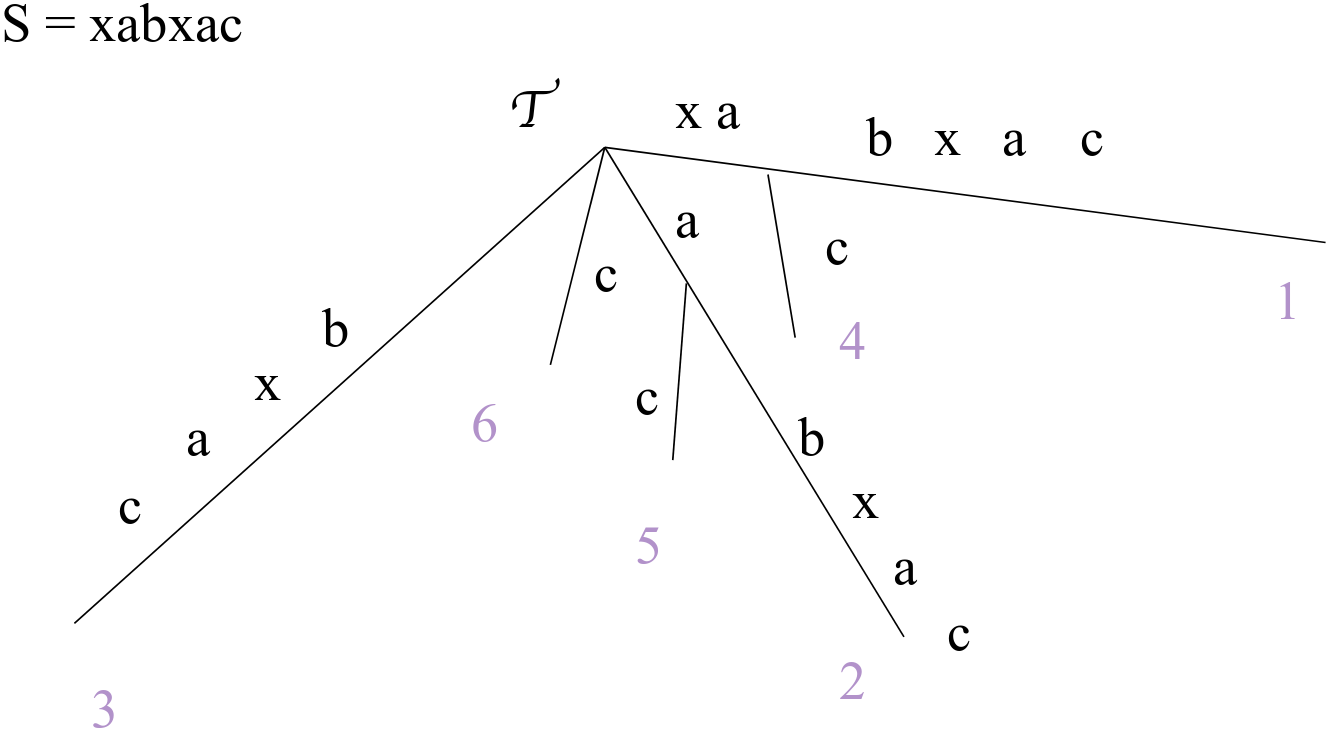
\includegraphics[width=0.9\textwidth]{img/suffix_tree.png}
		\caption{Example of suffix tree.}
		\label{f1}
	\end{minipage}
	\hspace{0.1cm}
	\begin{minipage}[t]{0.5\linewidth} 
		\centering
		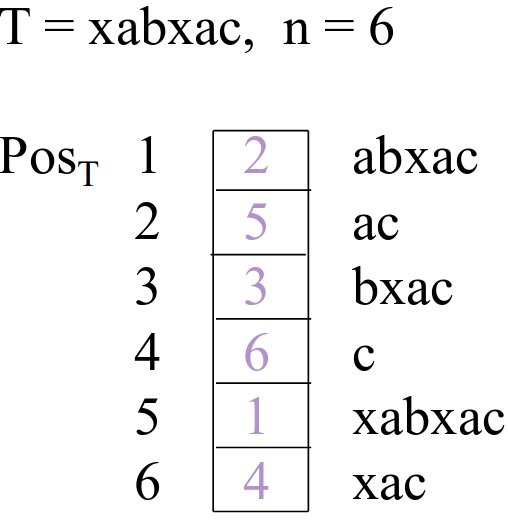
\includegraphics[width=0.5\textwidth]{img/suffix_array.png}
		\caption{Associated Suffix Array.}
		\label{f2}
	\end{minipage}        
\end{figure} 

Let us assume to have enough space to build the suffix tree for $T$ but not to save it permanently in memory. Then, Pos$_T$ can be obtained from the suffix tree for $T$ by \textit{traversing it "depth first in lexical order"}, with a time complexity $O(n)$. If in the suffix tree the sons of each node are already stored in lexical order, it is a simple depth-first traversing.

\subsection{Pattern matching with suffix array}
Once we have computed the suffix array the pattern matching algorithm is performed as follows:
\begin{itemize}
	\item if $P$ is contained in $T$, then all its occurrences are consecutive in Pos$_T$.
	$$\text{Ex:~P~=~xa}\quad \text{corresponds to Pos}_T[5]~=~1,\quad \text{Pos}_T~=~4$$
	\item In order to find the occurrences of $P$ in $T$ performs a binary search in Pos$_T$ comparing $P$ with the corresponding suffix of $T$:
	\begin{enumerate}
		\item with a binary search one can find the \textbf{first} occurrence of $P$ in Pos$_T$,
		\item with another binary search one can find the \textbf{last} occurrence of $P$ in Pos$_T$.
	\end{enumerate}
\end{itemize}
Complexity of the search of all the occurrences of $P$ of size $m$: $O(m~log~n)$, the worst case depends on how many long prefixed of $P$ are in $T$. Considering random strings we can have $O(m~+~log~n)$.
\image{img/searchPatternSuffixArray.png}{Search for a pattern}{0.6}
\subsection{mlr accelerator}
Let us assume there are many long prefixed of $P$ in $T$. We can optimize the pattern matching with the \textbf{mlr (minimum left right)} accelerator.
\begin{itemize}
	\item $L,R$ indicate the bounds of the search interval (at the beginning $L= 1$, $R = n$);
	\item $\mathcal{L}$ = length of the max common prefix between Pos$_T[L]$ and $P$.
	\item $\mathcal{R}$ = length of the max common prefix between Pos$_T[R]$ and $P$.
	
	$$Ex:\qquad P = xa,~ L = 4,~ R = 6 \quad \rightarrow \mathcal{L} = 0, \mathcal{R} = 2$$
	\item at each iteration in the binary search we inspect $M = \lceil\frac{L+R}{2}\rceil$.
	\item it is useless to compare $P$ with the prefix corresponding to Pos$_T[M]$ in the first mlr = min($\mathcal{L}, \mathcal{R}$) symbols. Then the comparison can start at symbol $mlr~+~1$
\end{itemize}

The cost of maintaining mlr is small, but it avoids many useless comparisons, optimizing the overall time complexity. The worst case is still $O(m~log~n)$, meaning that the symbols in $P$ from $mlr+1$ to $max(\mathcal{L}, \mathcal{R})$ are compared more than once.
Our goal is to reach a complexity equal to $O(m+log~n)$ also in the worst case, meaning that we need to reduce the number of useless comparison and any symbol in $P$ should be examined only once or a constant number of times.

\subsection{Super Accelerators Lcp}
It is possible to get $O(m+log~n)$ by using the super accelerators \textbf{Lcp(L,M)} and \textbf{Lcm(M,R)} besides $\mathcal{L}$ and $\mathcal{R}$ (more efficient, but more complex in the logic).\\


\paragraph{Definition.} $Lcp(i,j) = $ length of the longest common prefix between Pos$_T[i]$ and Pos$_T[j]$.
$$Ex:\qquad Pos_T[5]~and~Pos_T[6] ~\rightarrow~Lcp(5,6)~=~|xa|~=~2$$
For all $(L,M,R)$ we use $Lcp(L,M)$ and $Lcp(M,R)$ as accelerators, and note that Lcp values are defined on the text only, not on the pattern. Hence, they can be pre-computed and then used for pattern matching.

\paragraph{How to use accelerators.}

\begin{enumerate}
	\item \textbf{Simples case}: if $\mathcal{L} = \mathcal{R}(= mlr)$, then $P$ is compared with Pos$_T[M]$ starting at $mlr+1$, as in the algorithm with mlr accelerator.
	
	\item \textbf{General case}: $\mathcal{L} \neq \mathcal{R}$\\
	Let us assume $\mathcal{L} > \mathcal{R}$, that is $max(\mathcal{L},\mathcal{R}) = \mathcal{L}$ and $mlr = \mathcal{R}$. We can easily deduce that the symmetric case is reached when $\mathcal{L} < \mathcal{R}$, that is $max(\mathcal{L},\mathcal{R}) = \mathcal{R}$ and $mlr = \mathcal{L}$.\\
	Then we have $3$ different subcases:
	\image{img/superAccelerators.png}{How to use super accelerators}{0.8}
\end{enumerate}

\textbf{Property:} using the Lcp values, the search algorithm does at most $O(m~+~log~n)$ comparisons and runs in that time. For the proof look to the slides (pag 126).
The idea is that all symbols of $P$ are examined with $O(m)$ comparisons, there are at most $O(log~n)$ redundant comparisons, since for each iteration at most perform one redundant comparison (the last mismatch of $P$) and there are at most $O(log~n)$ iterations. So in total we can have a time complexity equal to $O(m~+~log~n)$.

\subsection{How to compute Super Accelerators}
Given a text of length $n$, the $Lcp$ values need to be pre-computed before using them for pattern matching. The time complexity of this operation is $O(n)$. For example, consider $n= 2^k$ and let $B$ the binary tree corresponding to all possible search interval, so that is has $n(n-1)$ nodes:
\image{img/LR.png}{B binary tree with $n(n-1)$ nodes}{0.7}

\textbf{Property:} Let $\mathcal{T}$ be the suffix tree for $T$ and $\varphi$ be the set of internal nodes traversed from the Pos$_T[i]$ and the leaf Pos$_T[i+1]$ during the lexical depth-first traversal. Let $v$ be the node in $\varphi$ closest to be root and let $\gamma$ be its label (the associated string), then $Lcp(i, i+1) = |\gamma|$.

\image{img/lcp.png}{Lexically ordered suffix tree}{0.8}
The algorithm used to compute the $Lcp(i, i+1)$:
\begin{itemize}
	\item $Lcp(i, i+1)$ can be computed while building the suffix array;
	\item The suffix tree can be built by annotating each node with its string depth 
	\item Then, the values $Lcp(i, i+1)$ can be computed by a lexical depth-first traversal of the suffix tree, while building the suffix array $ \rightarrow ~ O(n)$
	\item Let $\mathcal{L}_1$ be the traversed leaf and $\mathcal{L}_2$ the next leaf, if it exists, let us indicate $Lcp(\mathcal{L}_1,\mathcal{L}_2)$ with $Lcp(\mathcal{L}_1)$:
	\begin{itemize}
	\item if $\mathcal{L}_1$ has a right brother in the lexicographic order, then $Lcp(\mathcal{L}_1)$ is the string depth associated to their father node;
	\item If $\mathcal{L}_1$ is the last son, then $Lcp(\mathcal{L}_1)$ is the string depth of the closest predecessor of $\mathcal{L}_1$ which has further sons;
	\item if $\mathcal{L}_1$ is the last leaf, then $Lcp(\mathcal{L}_1) = 0$;
	\image{img/superAcceleratorProperty}{Property}{0.5}
	\end{itemize}

	\item In the binary tree $B$ (representing the search intervals), by associating the $Lcp(i,i+1)$ to the leaves, it is possible to compute the $Lcp(i,j)$, for $j~>~i+1$, by walking up from the leaves and setting the Lcp value at any node $v$ to the minimum of the Lcp values of its two children;
	\item Tree traversal requires visiting all nodes: $2n-1\quad \rightarrow ~ O(n)$.
\end{itemize}
\chapter{Pair Alignment}
\section{Alignment}
Alignment refers to the proper positioning or state of adjustment of parts (as of a mechanical or electronic device) in relation to each other.
It is a fundamental technique in bioinformatics and often it represents the first step in many evolutionary and functional studies. Errors in alignment tend to amplify in later computational stages.\\
In general we talk about alignment of sequences and there are essentially two reasons for which it is very useful:
\begin{itemize}
	\item \textbf{Studying function}, sequences that are similar probably have similar functions;
	\item \textbf{Studying evolution}, similarity is mostly indicative of common ancestry;
\end{itemize}
\image{img/ancestor.png}{Common ancestor example}{0.5}

\subsection{Homology}
Two important concepts used in bioinformatic are related to the notion of \textbf{homology} and \textbf{analogy}.\\

\textbf{A is Homologous to B} if they are related by divergence from a common ancestor. Then we can find another division of this family:
\begin{itemize}
	\item Paralogues, different but related functions in one organism.
	\item Orthologues, same function in different organisms.
\end{itemize}

\textbf{A is Analogous to B} if they gave a similar function but possibly different origins. Different sequence with the same structure may have common ancestor, instead different sequence with different structure may be convergent to evolution.\\

Now we define $4$ operators that can change a sequence:
\begin{figure}[h]
	\begin{minipage}[t]{0.5\linewidth}
		\centering
		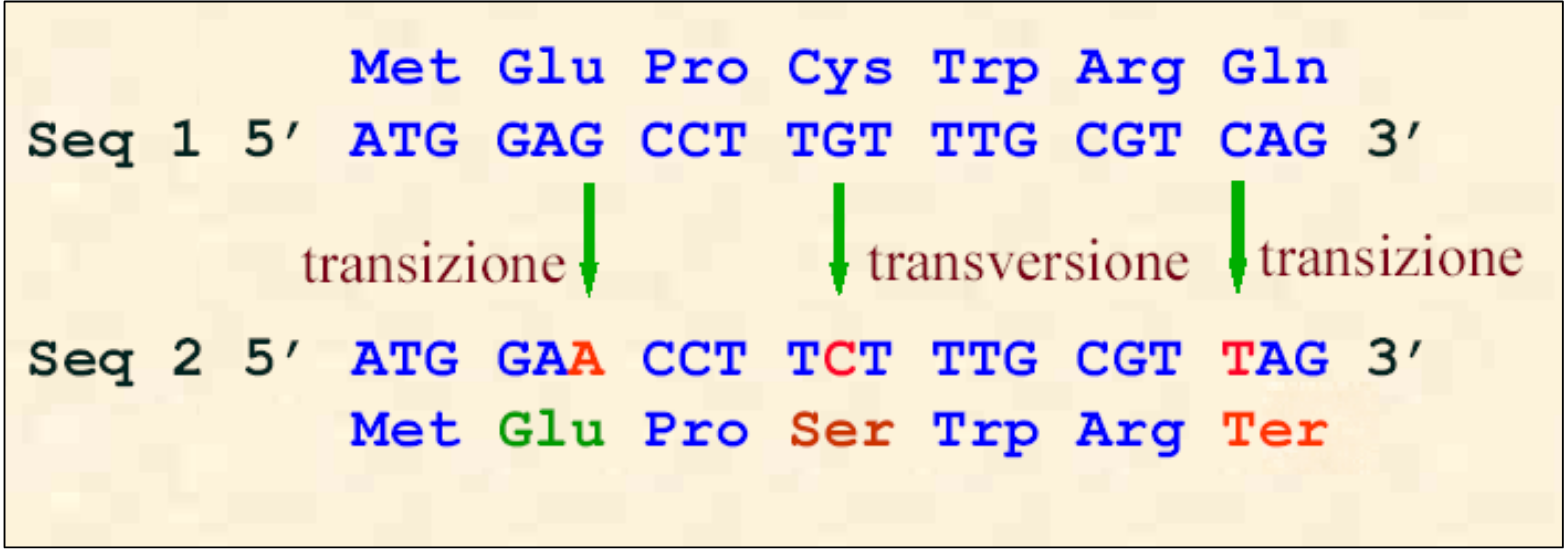
\includegraphics[width=0.9\textwidth]{img/mutation.png}
		\caption{Mutation operator.}
		\label{f1}
	\end{minipage}
	\hspace{0.1cm}
	\begin{minipage}[t]{0.5\linewidth} 
		\centering
		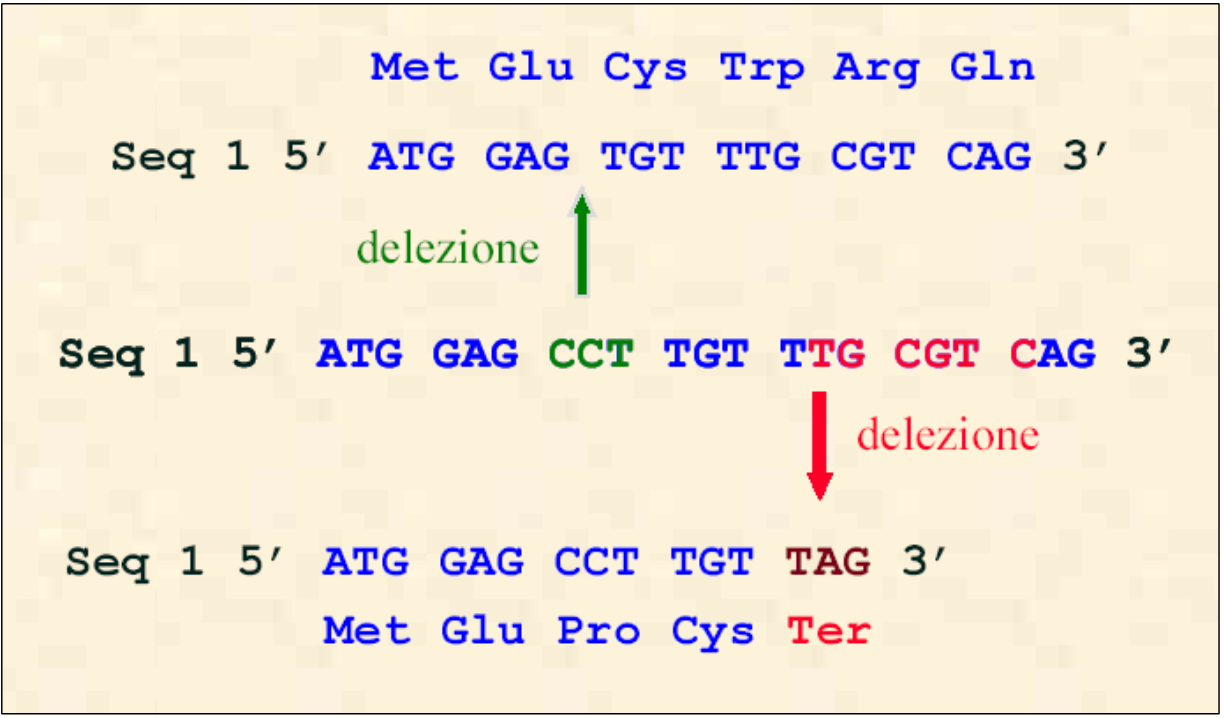
\includegraphics[width=0.9\textwidth]{img/deletions.png}
		\caption{Deletion operator.}
		\label{f2}
	\end{minipage}        
\end{figure} 

\begin{figure}[h]
	\begin{minipage}[t]{0.5\linewidth}
		\centering
		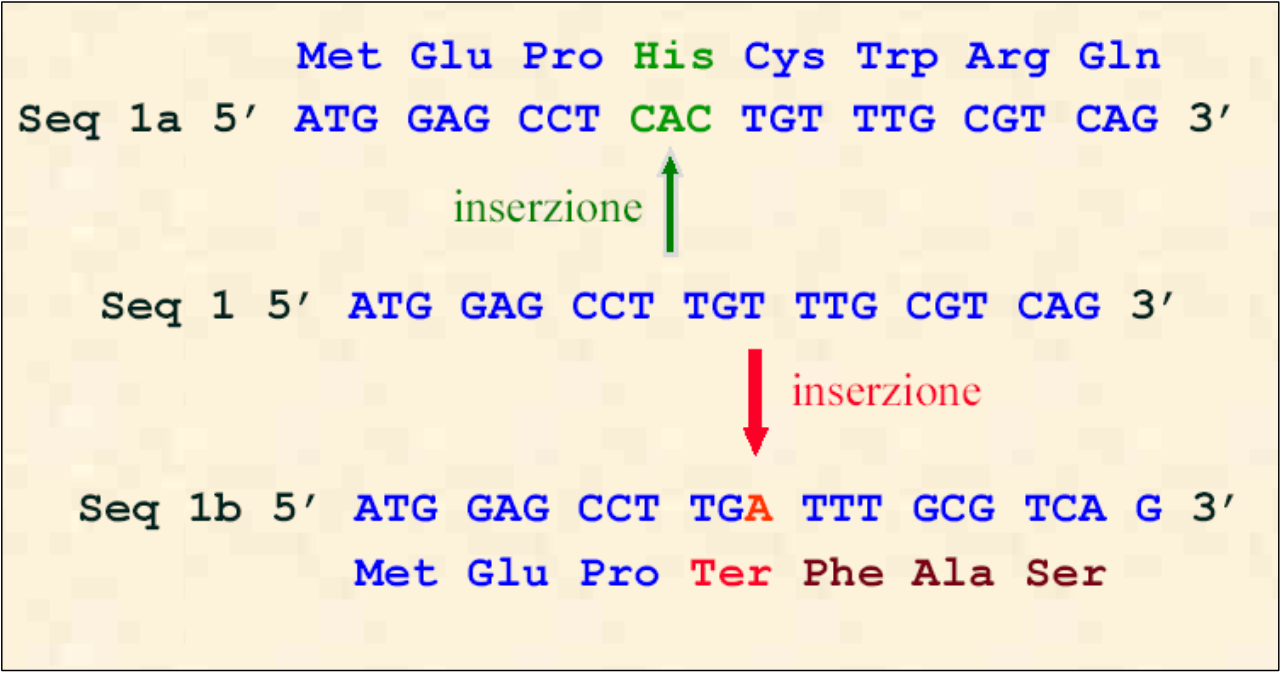
\includegraphics[width=0.9\textwidth]{img/insertions.png}
		\caption{Insertion operator.}
		\label{f1}
	\end{minipage}
	\hspace{0.1cm}
	\begin{minipage}[t]{0.5\linewidth} 
		\centering
		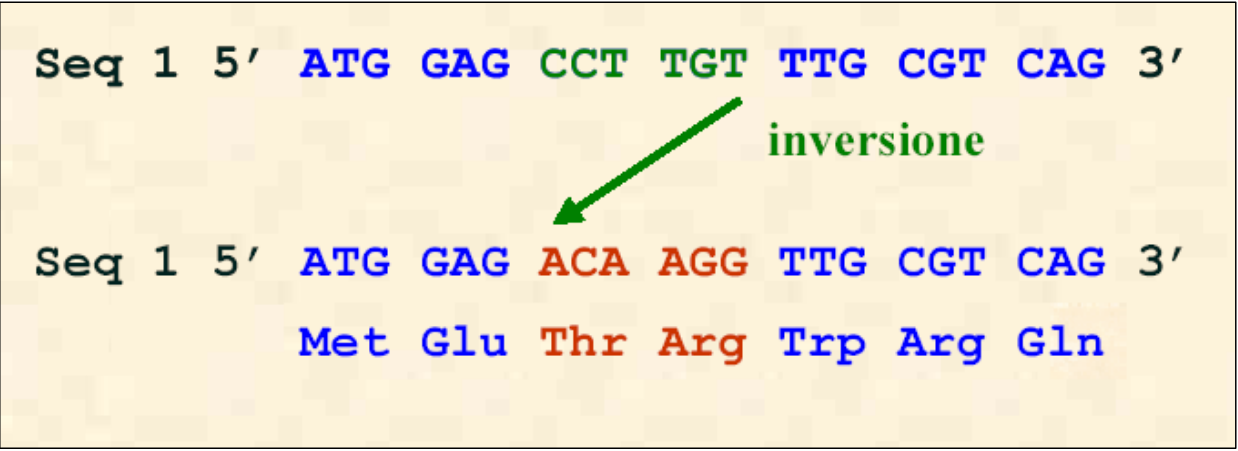
\includegraphics[width=0.9\textwidth]{img/inversions.png}
		\caption{Inversion operator.}
		\label{f2}
	\end{minipage}        
\end{figure} 
\image{img/omologia.png}{Homologous sequences}{0.5}


\section{Sequence Alignment}
Sequence alignment would require the identification of the correct location of \textit{deletions} and \textit{insertions} that have occurred in either of the two lineages since their divergence from a common ancestor. This never happens, it is impossible, but we can check for the \textbf{maximal parsimony hypothesis}, which is an optimal criterion under which the phylogenetic tree that minimizes the total number of character-state changes is to be preferred.\\
When we talk about alignment we should take in consideration different things like: type of alignment, allowing gaps, score system, algorithm and evaluation of the results.

\subsection{Type of Alignment - 1.}
Two main types of alignment:
\begin{itemize}
	\item \textbf{Global alignment}, compares the whole sequence $A$ with the whole sequence $B$. It is used in comparative and evolutionary studies.
	
	\item \textbf{Local alignment}, determines if sub-segments of one sequence ($A$) are present in another ($B$). It finds its greatest utility in database searching and retrieval. 
\end{itemize}
When we have biological sequences that are distant from each other it could be difficult to obtain a correct alignment in regions of low similarity. Local alignment avoids such regions altogether and focuses on those with a positive score, i.e. those with an evolutionary conserved signal of similarity.

\subsection{Type of Alignment - 2.}
Sequence alignment may be divided into two categories:
\begin{itemize}
	\item \textbf{Pairwise alignment}, alignment of two sequences. This problem has \textit{exact solution}.
	\item \textbf{Multiple-sequence alignment}, alignment of three or more sequences. It is not exact solved, but there exist some approximate (heuristic) solutions.
\end{itemize}

\subsection{Gaps}
There are \textbf{internal} and \textbf{terminal} gaps.
\image{img/gaps.png}{Type of gaps.}{0.6}
\begin{itemize}
	\item \textbf{Internal}, they are located inside the string and they may indicate that a deletion or an insertion has occurred in one of the two lineages.
	\item \textbf{Terminal}, they are located on the external sides of the string and they may indicate missing data.
\end{itemize}

\subsection{Methods of alignment}
Alignment can be performed in different ways:
\begin{itemize}
	\item Manual
	\item Dot matrix
	\item Exact alignment
	\item Heuristic (word methods)
\end{itemize}

\subsubsection{Manual Alignment}
When there are few gaps and the two sequences are not too different 
from each other, a reasonable alignment can be obtained by 
\textbf{visual inspection}. 

\subsubsection{Dot matrix}
The two sequences are written out as column and row heading of two-dimensional matrix. A \textbf{dot} is put in the dot-matrix plot at a position where the nucleotides in the two sequences are identical. Then we can distinguish $4$ different cases:
\begin{itemize}
	\item \textbf{match}, indicated by a diagonal step through a dot. (Diagonal step from a cell to another one which have a dot)
	
	\item \textbf{mismatch}, indicated by a diagonal step through an empty element of the matrix. (Diagonal step from a cell to another one which is empty)
	
	\item A \textbf{gap} in the sequence used in column (on the top of the matrix), indicated with a vertical step
	
	\item A \textbf{gap} in the sequence used in row (on the left of the matrix), indicated with a horizontal step.
\end{itemize}
\image{img/dot_matrix.png}{Dot matrix between two biological sequences.}{0.4}
An interesting property of the dot matrix is that it allows to find also palindrome strings looking for opposite diagonals.

The main problem of this visualization tool is that when we have long sequences the dot matrix became not easy to understand. With long sequences (like DNA sequences) the matrix becomes cluttered. In order to improve its readability the \textbf{sliding window} technique is adopted, which is based on the idea of collapsing the dots in the original dot matrix. The sliding window procedure consists on defining a matrix $k\times k$ and starting from the first position on the dot matrix check if there are at least $h$ dots inside the window. In case of positive match a new dot in the center of the window is included in the new dot matrix. Otherwise no dots are included. The parameters $k$ and $h$ are called \textbf{windows size} and \textbf{stringency} respectively. The main advantage of this procedure is that changing the values of $k$ and $h$ we can project the original dot matrix in different scales and have different views on data (\textbf{trial-and-error}).

\image{img/dotMatrixSliding3.png}{Dot matrix example with sliding window $k = 3$ and $h = 2$.}{1}

\textbf{Advantages} of dot matrix:
\begin{itemize}
	\item It is simple to implement.
	\item Trial-and-error procedure to have different views on data. It can be useful since it may unravel information on the evolution of sequences or it may be used to compare one sequence to itself and study repetitions. 
\end{itemize}

\textbf{Disadvantages} of dot matrix:
\begin{itemize}
	\item Expensive for large sequences analyses.
	\item It may not identify the best possible alignment.
	\item Qualitative view, either match or mismatch, no quantification with a similarity score.
\end{itemize}

\subsubsection{Exact and Heuristic}
The true alignment between two sequences is the one that reflects accurately the evolutionary relationship between the sequences. Since the \textbf{true alignment} is unknown, in practice we look for the \textbf{optimal alignment}, which is the one in which the number of mismatches and gaps are minimized according to a certain criteria (depending on the score).\\

In order to determine an optimal alignment we need to choose a scoring system, which comprises a \textbf{gap penalty} and a \textbf{scoring matrix} $M(a,b)$ that specifies the score for each type of match (a = b) or mismatch (a $\neq$ b). 

Extra: The units in a scoring matrix may be the nucleotides in DNA or RNA sequences, the codons in protein-coding regions, or the amino acids in protein sequences.\\

Mismatch and gap penalties should be \textit{inversely proportional to the frequencies} with which changes occur. Scoring matrices are based on the \textit{additive property of the score} meaning that it implies position independence and the score can be calculated by scrolling the string.
\newpage
\subsubsection{Scoring matrices for DNA}
DNA scoring matrices are usually simple, since all mismatches are given the same penalty:
$$M(a,b) = \begin{cases}
>~0 & \text{if}~a = b\\ 
\leq~0 & \text{if}~a \neq b\\
\end{cases}$$
In more complicated matrices a distinction may be made and each type of mismatch may be penalized differently.

\subsubsection{Scoring matrices for Aminoacids}
For aminoacids we can distinguish among different matches and mismatches. Example: a mismatched pair consisting of $Leu~\&~lle$, which are very similar biochemically to each other, may be given a lower penalty than a mismatched pair consisting of $Arg~\&~Glu$, which are very dissimilar from each other.

\subsection{Gap Penalties}
\textbf{Gap penalty} (or cost) is a factor (or a set of factors) by which the gap values (numbers and lengths of gaps) are multiplied. The gap penalties are based on our assessment of how frequent different types of \textit{insertions} and \textit{deletions} occur in evolution in comparison with the frequency of occurrence of point substitutions.\\
The gap penalty may have two components:
\begin{itemize}
	\item a gap-opening penalty
	\item a gap-extension penalty
\end{itemize}

In literature we have different systems for gap penalty:
\begin{itemize}
	\item \textbf{Fixed gap-penalty system}, example $0$ gap costs.
	\item \textbf{Linear gap-penalty system}, the gap cost is calculated by multiplying the gap length $g$ by a costant $d$: $\gamma(g) = -gd$.
	\item \textbf{Affine score}, it distinguishes a gap-opening cost $d$ and a gap-extension cost $e$: $\gamma(g) = -d - (g-1)e$, with $e~<~d$.
	
	\item \textbf{Logarithmic gap-penalty system}, the gap-extension penalty increases with the logarithm of the gap length (slower).
\end{itemize}

\image{img/logGap.png}{Gap penalty.}{0.6}

\image{img/effectOfGap.png}{Effect of gap penalties on amino acid alignment.}{0.8}

\subsection{Scoring matrices: Log-odds ratios}
A scoring matrix is a table of values that describes the probability of an amino acid pair to occur in an alignment. The values in a scoring matrix are \textbf{log rations of two probabilities},  meaning that:
\begin{itemize}
	\item One is the random probability (denominator);
	\item The other is the probability of a empirical pair occurrence (numerator);
\end{itemize}
The scores are logarithms of probability ratios, hence they can be added to give a meaningful score for the entire alignment. \textit{The more positive the score, the better the alignment}.\\
Let $x = x_1 \dots x_n$ and $y = y_1 \dots y_n$ be the pair of sequences to align (for simplicity no gap), it is possible to define:

\paragraph{Probability of the random alignment:} $P(x,y|R) = \Pi_{i = 1,n}{q_{xi}}~ \Pi_{j = 1,n}{q_{y_j}}$  \\
where $q_{xi},~q_{yj}$ are the probabilities of the symbols $x_i$ and $y_j$.

\paragraph{Probability of being correlated:} $P(x,y|M) = \Pi_{i = 1,n}{q_{x_iy_i}}$  \\

\textbf{Ratio}: $\frac{(P(x,y|M))}{P(x,y|R)} = \frac{\Pi_{i = 1,n}q_{x_iy_i}}{\Pi_{i = 1,n}q_{x_i} \Pi_{j=1,n}q_{y_j}} = \Pi_{i = 1,n}\Big[\frac{q_{x_iy_i}}{q_{x_i}q_{y_i}}\Big]$
where $q_{ix},~q_{yj}$ are the probabilities of the symbols $x_i$ and $y_j$.\\

\textbf{Log}: $\sum_{i = 1,n} \log(\frac{q_{x_iy_i}}{q_{x_i}q_{y_i}})$ in general multiplied by $10$ to get an integer.
\newpage
\subsection{Empirical substitution matrices}
\begin{itemize}
	\item \textbf{PAM} (Percent/Point Accepted Mutation) matrices assume a model where amino acid substitutions, observed at great evolutionary distances, it is the sum of many independent mutations. Hence, the \textit{PAM scores express the likelihood that the pairing of a pair of amino acids is due to homology rather than to the case.} PAM matrices are built through homologous sequences that represents only the 1\% of accepted mutations, where for "accepted" it is meant mutations that don't alter the protein function.\\
	\textbf{PAM1} matrix is the amount of evolutionary change that yields one substitution in 100 amino acids residues. To derive a mutational probability matrix for a protein sequence that has 	undergone N percent accepted mutations, a \textbf{PAM-N} matrix, the	PAM-1 matrix is multiplied by itself N times.

	\item \textbf{BLOSUM} (BLOcks SUbstitution Matrix) matrices do not make any homology assumption: the considered blocks are obtained by direct observation of the proteins having similar functions.
\end{itemize}

PAM matrices work but they have some disadvantages:
\begin{itemize}
	\item Assumed regular time in evolution;
	\item Assumed same evolutive speed for different species;
	\item No gap is considered;
	\item The phylogenetic tree is inferred;
	\item Simplifying assumptions in the computation of the scores: symmetry, reversibility and independence from position;
\end{itemize}

BLOSUM matrices are based on local alignments ("blocks" or conserved amino acid patterns). All BLOSUM matrices are based on observed alignments and they are not extrapolated from comparisons of closely related proteins. BLOSUM\textit{n} is based on sequences that are at most $n$ percent identical.

\paragraph{Comparison between PAM and BLOSUM.} Both of them are scoring matrices that define the penalties to apply in case of mismatch, but they tend to favor different behaviors. In particular PAM tends to favor homology and BLOSUM tends to favor functionalities.

\chapter{Pair alignment - Methods}
\section{Approximated Pattern Matching}
Consider the match between a text $T$ and a pattern $P$ with the possibility of having \textit{errors} both in the pattern and in the text. We can define a \textbf{similarity/distance between strings}. Ex: $aab$ is similar to $aac$? We need a \textbf{threshold} to distinguish when the comparison is meaningful.\\
Having a similarity measure between strings can be useful for different applications like: finding typos in texts, signal recovery with noise, finding similar strings in DNA or proteins, comparing two sequences. \\

Difference between strings is given by in terms of length and of symbols that they have. We can think that difference between strings can be expressed in the type and number of transformation is required to transform one string into the other one. There are $4$ operations that can be applied to modify strings:
\begin{itemize}
	\item \textbf{Insertion}, insert a symbol into the string; $Ex:~ aaa~\rightarrow~aaba$
	\item \textbf{Deletion}, eliminate a symbol from the string: $Ex:~ aaba~\rightarrow~aaa$
	\item \textbf{Substitution}, substitute a symbol with another one in the string; $Ex:~ aaba~\rightarrow~aaca$
	\item \textbf{Transportation}, switch the order of two adjacent symbols in the string; $Ex:~ aaba~\rightarrow~aaab$
\end{itemize}
These operations are associated to a \textbf{cost}, that can be:
\begin{itemize}
	\item They may have the same cost (\textit{constant});
	\item Different cost for each operation;
	\item Even a different cost for each symbol (\textit{penalty matrices}).
\end{itemize}

\section{Distance between two strings}
Let $A$ and $B$ be two strings, their \textbf{distance} $d(A,B)$ is the minimal cost of a sequence of operations which transform $A$ into $B$. If there is not such a sequence of transformations the cost is infinite $(\infty)$.
$$Ex:~A~=~POLITE,~B=~PLATE$$
$$\text{POLITE}~\rightarrow \text{delete(2)},~ \text{substitution(3,A)}~\rightarrow~\text{PLATE}$$
This is the minimal sequence of operations considering, and if we fix that the cost of each operation is $1$ then the distance is $2$.\\
On the rest of this section we are going to propose different distance metrics for comparing strings.

\subsection{Hamming Distance}
It permits only substitutions for computing distance between strings. It is symmetric and not transitive: $\text{if }|A|~=~|B|,~ 0\leq d(A,B) \leq |A|$.\\

$\text{Ex: X = aaaccd, Y =abcccd}$\\
$d(X,Y)~=~2 \quad \text{since at least two substitutions are necessary.}$

\subsection{Levenshtein(Edit) Distance}
It permits the usage of more transformation operation respect to the hamming distance, which consider only substitutions. The edit distance, in fact, takes in consideration insertions, deletions and substitutions. It is symmetric and has the following property:
$$0 \leq d(A,B) \leq max(|A|,|B|)$$
$$\text{EX: X = aaaccd, Y = abccd}$$
$$d(X,Y) = 2 \quad \text{since at least a substitution and a deletion are necessary.}$$

\subsection{Episode Distance}
It permits only insertions and it isn't symmetric. Since it consider only insertions it is possible that $A$ and $B$ cannot match through transformation, meaning that $d(A,B)= \infty$. Otherwise in the other cases we have that $d(A,B)=|B|-|A|$.

$$\text{EX: X = aaccd, Y = abbaccd}$$
$$d(X,Y) = 2 \quad \text{since two insertions are necessary.}$$

\section{Similarity between two strings}
Let $d$ be a distance and $e$ be an error threshold, then we can define a \textbf{similarity relation between strings}, $\sim_e$:
$$A\sim_eB \qquad d(A,B)\leq e$$
This concept extends the equality relation between strings and in general it is not transitive and it may not be symmetric.


\section{Pair Alignments}
An alignment between a string $A$ with $n$ symbols and a string $B$ with $m$ symbols is an array $L$ of dimension $2\times max(n,m)$, in which:
\begin{itemize}
	\item the first row contains the symbols of $A$ or $\varepsilon$;
	\item the second row contains the symbols of $B$ or $\varepsilon$;
\end{itemize}
so that by eliminating $\varepsilon$ one can obtain $A$ and $B$ again. 

\image{img/globalAlignment.png}{Global Alignment.}{0.6}
From the previous example we have seen that for two strings we can have multiple available alignments. In general we have a fixed number of alignments:
$$\binom{n+m}{min(n,m)} = \frac{(n+m)!}{n!m!}\approx \sqrt{\frac{n+m}{2\pi nm}}\times \frac{(n+m)^{(n+m)}}{n^n\times m^m}$$
where $n$ and $m$ are the lengths of the two sequences to be aligned.

\subsection{Optimal Alignment}
An optimal alignment is an alignment in which the \textbf{distance} between the two strings is \textbf{minimal} (or the similarity is maximal).
\image{img/optimalAlignment.png}{Optimal Alignment example.}{0.6}

\subsection{Back to Approximated Pattern matching}
The problem of the Longest Common Subsequence (LCS) of two given sequences consists on: given a similarity relation between strings $\sim_e$ it is possible to search for strings similar to a pattern $P$ in a text $T$. We need a method to compute the minimal distance/maximal similarity between two strings (the optimal alignment) and a method to search the substrings similar to $P$ in $T$.


\subsection{Exact Optimal Alignment Algorithms}
Optimal alignment can be reached with different algorithms:

\paragraph{Dynamic programming.} Let $A$ and $B$ two strings of length $n$ and $m$, respectively, then we define $D(i,j)$ as the edit distance between $A[1\dots i]$ and $B[1\dots j]$. In other words $D(i,j)$ denotes the minimum number of edit operations needed to transform $A[1\dots i]$ into $B[1\dots j]$.\\
Edit operations are:
\begin{itemize}
	\item insertion of a character;
	\item deletion of a character;
	\item substitution of a character;
\end{itemize}
Hence the edit distance of $A$ and $B$ is the value $D(n,m)$. We use a dynamic programming approach to compute $D(n,m)$, which is composed by three main components:
\begin{enumerate}
	\item \textbf{Recurrence relation}, establish a recursive relation between the value of $D(i,j)$ with $i,j$ positive, and values of $D$ for index pairs smaller than $i$ and $j$;
	\item \textbf{Tabular computation}, uses the recursive relation to efficiently compute $D(n,m)$. There can be applied two types of approaches. \textit{Top-down approach} using recursion, but it is not efficient. The \textit{bottom-up approach} first compute $D(i,j)$ for the smallest possible values and then compute $D(i,j)$ for all the choices of $i$ and $j$.
	\item \textbf{Traceback}, once all values of $D$ have been computed, extract an optimal solution;
\end{enumerate}

\image{img/editDistanceInductive.png}{Edit distance: inductive definition.}{0.5}

\paragraph{Needleman-Wunsch Algorithm}
The Needleman-Wunsch algorithm allows to build the edit distance table given in input two strings $A$ and $B$, with dimension $n$ and $m$. It assumes that the cost of each operation is $1$ and produces in output a table $D$, $n\times m$, containing the values of the \textbf{edit distance} and the links.  $D$ is inductively defined with respect to the indexes.

\image{img/needlemanWunsch.png}{Needleman-Wunsch Algorithm to build the edit distance table.}{0.5}

When the value of $D[i,j]$ is computed, set a pointer (one or more) from $D(i,j)$ to :
\begin{itemize}
	\item $D[i-1, j-1]$ if $D[i,j] = D[i-1,-1] + f(i,j)$;
	\item $D[i, j-1]$ if $D[i,j] = D[i,j-1] + 1$ (horizontal step);
	\item $D[i-1, j]$ if $D[i,j] = D[i-1,j] + 1$ (vertical step);
\end{itemize}
For cells in row $0$ or column $0$ set a pointer to the only possible direction. The pointers allow for an easy recovery of an optimal edit transcript from $A$ to $B$: simply follow any path of pointers from cell $D[n,m]$ to cell $D[0,0]$:
\begin{itemize}
	\item a vertical step corresponds to aligning a symbol in $A$ with a gap in $B$;
	\item a horizontal step corresponds to aligning a symbol in $B$ with a gap in $A$;
	\item a diagonal step corresponds to a match or a mismatch.
\end{itemize}

\image{img/computingPointers.png}{Example of computing pointers.}{0.5}

The complexity of N-W:
\begin{itemize}
	\item Space: $S(nm)$ which is required to store $D$.
	\item Time for building $D$: $O(nm)$;
	\item Time for tracing back an optimal alignment: $O(n+m)$; 
\end{itemize}

\image{img/needleman-wunsch.png}{Example of Needleman-Wunsch Algorithm.}{0.6}

\paragraph*{Inductive definition of the similarity score.} The similarity score can be obtained also through an inductive definition where $D[i,j]$ is the score of the optimal alignment between $A[1 \dots i]$ and $B[1 \dots j]$.\\
\image{img/inductive_definition}{Inductive definition of the similarity score.}{0.55}
Thanks to this definition it is possible to define the N-W algorithm.

\subsection{Semiglobal Alignments}
Semiglobal alignment is useful when one sequence is short (for example a gene sequence) and the other is very long (for example a chromosome sequence). In that case, the shortest sequence should be globally aligned but only a local alignment is desired for the long sequence. The shortest sequence is aligned through the introduction of external gaps that can allow the pre-computation of specific rows/columns of the resulting table.
\image{img/semiglobal1}{Semiglobal Alignments.}{0.7}
\image{img/semiglobal2}{Semiglobal Alignments.}{0.7}
The application of this improvement makes possible for us to determine the following algorithm:
\image{img/edit_distance_inductive}{Semiglobal Alignment: Edit Distance Inductive Definition.}{0.55}

\subsection{Approximated Pattern Matching}
It is possible to notice the fact that semiglobal alignment is similar but not equal to an approximated pattern matching, indeed, the pattern is usually much shorter than the text.\\
We can consider a problem where:
\begin{itemize}
	\item \textbf{Input:} a pattern $P$ of size $m$, a text $T$ of size $n$ and an error threshold $\delta$ (Each operation costs 1 and match costs 0).
	\item \textbf{Output:} a table $D$ of size $m \times n$ containing the edit distance.
\end{itemize}
With these premises, it is possible to define the approximated pattern matching algorithm through the building of the distance table $D$.
\image{img/approximated_pattern_matching}{Approximated pattern matching: building of the distance table.}{0.55}
This algorithm produces the following table:
\image{img/approximated_pattern_matching_table}{Table created with the approximated pattern matching algorithm.}{0.55}
In order to find possible occurrences of $P$, we can notice that any $D[m,j] \leq \delta$ corresponds to an approximated occurrence of $P$. In a more detailed way:
\image{img/occurences_P}{Procedure used to find approximated occurrences of $P$.}{0.55}

\subsection{Comparison between global/local alignment.} Global and local alignment are used for different purposes indeed:
\begin{itemize}
	\item \textbf{Global alignment} is used for sequences comparison.
	\begin{center}
		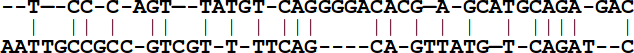
\includegraphics[width=0.5\textwidth]{img/global}
	\end{center}
	\item \textbf{Local alignment} allows to find conserved motifs.
	\begin{center}
	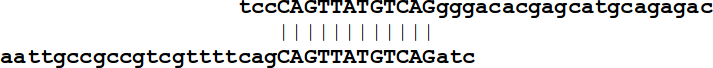
\includegraphics[width=0.5\textwidth]{img/local}
	\end{center}
\end{itemize}

\paragraph*{Smith-Waterman Algorithm.} The initial scoring matrix of S-W enables the alignment  of  any segment of one sequence to an arbitrary position in the other sequence. It can do this because of the fact that no negative score is assigned in the scoring system.\\
This algorithm has the following properties:
\begin{itemize}
	\item It enables local alignment.
	\item When any element has a score lower than 0, it means that the sequences up to this position have no similarities. This element will then be set to 0 to eliminate influence from previous alignment.
	\item In this way, calculation can continue to find alignment in any position afterwards.
\end{itemize}
The distance table $D$ is created through the following procedure:
\image{img/SW1}{S-W: similarity score between two sequences.}{0.6}
As it is possible to see, the procedure is applicable also when scores can be negative. The S-W algorithm has the following input/output:
\begin{itemize}
	\item \textbf{Input:} two sequences to be aligned \textbf{A} and \textbf{B}, a threshold for the minimal score $\delta$.
	\item \textbf{Output:} a table $D$, $m \times n$, containing the values of the similarity score.
\end{itemize} 
The S-W algorithm is described as follows:
\image{img/SW2}{S-W algorithm.}{0.6}
The resulted scoring table (with match = +1, mismatch/gap=-1) can be observed below:
\image{img/SW3}{Resulting table.}{0.6}
The previous table is used in order to find local alignments. If $D[i,j] \geq \delta$ and in the next cells (adjacent lower and to the right) the score is smaller, we have a local optimal alignment. In other words, it starts from such a $D[i,j]$ and then it traverses the table towards up and left (following the pointers), up to a cell with score 0.\\
The choice of the alignments (many could be produced in general) depends on the application.
\begin{center}
	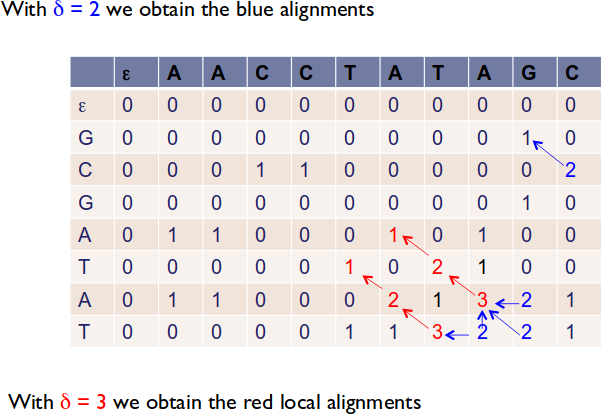
\includegraphics[width=0.73\textwidth]{img/SW4}
\end{center}

\paragraph*{Comparison between N-W and S-W.} Easily it is possible to differentiate the two algorithms according to their purposes:
\begin{itemize}
	\item \textbf{S-W} finds the segments in two sequences that have similarities.
	\item \textbf{N-W} aligns two complete sequences.
\end{itemize}
However they can be compared surely through their similarities and their differences. Both the algorithms use the concepts of a substitution matrix, a gap penalty function, a scoring matrix and a traceback process. On the other hand, they present also several differences:
\begin{table}[H]
	\centering
	\begin{tabular}{| p{2.5cm} | p{5.5cm} | p{5.5cm}|}
		\hline
		 & \textbf{S-W algorithm} & \textbf{N-W algorithm} \\
		 \hline
		 \textit{Initialization} & First row and first column are set to 0. & First row and first column are subject to gap penalty.\\
		 \hline
		 \textit{Scoring} & Negative score is set to 0. & Score can be negative. \\
		 \hline
		 \textit{Traceback} & Begin with the highest score, end when 0 is encountered. & Begin with the cell at the lower right of the matrix, end at top left cell.\\
		\hline
	\end{tabular}
	\caption{Differences between S-W and N-W.}
\end{table}

\subsection{Heuristic Methods.}
They are much faster than exact methods (N-W, S-W) that usually require a time complexity of $O(n^2)$. The drawback of these heuristic methods is that they do not guarantee to find the optimal alignment.

\paragraph*{MUMmer.} \textit{Maximal Unique Matches} (MUMs) is identified in two sequences by a generalized suffix tree. The purpose is to find the longest increasing sequences of MUMs without crossing.
\image{img/MUMs}{MUMmer representation.}{0.75}

\paragraph*{FASTA.} It is 10 times faster than S-W, it is considered as an accurate tool especially for sequences with repetitions (DNA). The algorithm is divided in the following steps:
\begin{itemize}
	\item Split the query into words (DNA ktup=4 or 6, proteins	ktup=1 or 2).
	\item Build a lookup table which shows the positions in the query for each word (\textit{indexing the query}).
	\item Build a lookup table also for the target sequence, which shows the shifts with respect to the query (\textit{indexing the target}).
	\item Determine the best similarities by comparing the shifts (\textit{Init1}: diagonals).
	\item Extend close diagonals with gaps (\textit{InitN}) like a dot-plot.
	\item Apply \textbf{Smith-Waterman} to the diagonals.  
\end{itemize}

\paragraph*{BLAST.} It stands for Basic Local Alignment Search Tool and it is 50 times faster than S-W. BLAST is the nowadays standard tool for local sequence similarity searching. It follows these steps:\\
Given a query sequence and a sequence DB:
\begin{itemize}
	\item Split the query into words of length W (4 or 3) by a \textbf{sliding window} of size W.
	\item For each word generate a list of similar words called \textbf{W-mers} with similarity score greater than T (global alignment using N-W).
	\image{img/BLAST}{BLAST step 2.}{0.5}
	\item Find good local alignments of words into DB (\textbf{seeds}) (\textbf{one hit method}). 
	\image{img/BLAST2}{BLAST step 3.}{0.5}
	\item Extend the \textbf{hit} on both sides without gap, up to a score threshold S (without applying S-W, it only recomputes the score).
	\item If the score is negative, \textbf{X} specifies how much to insist on extending the alignment.
		\image{img/BLAST3}{BLAST step 5.}{0.5}
\end{itemize}

\paragraph*{FASTA vs BLAST.} Between these two algorithms, we can find the following differences:
\begin{table}[H]
	\centering
	\begin{tabular}{| p{7cm} | p{7cm}|}
		\hline
		\textbf{FASTA} & \textbf{BLAST} \\
		\hline
		\textit{Init1} is determined through identity, hence it can miss the optimal alignment. & Generally gaps are not inserted.\\
		\hline
		It is better for DNA-RNA. & It is better for proteins (similarity, not exact match). \\
		\hline
	\end{tabular}
	\caption{Differences between FASTA and BLAST.}
\end{table}

\subsection{Results Evaluation.}
Given an alignment of a query sequence A with a sequence B with score S, it is necessary to ask what does it mean this result?\\ 
In a set of random sequences, how much is the probability to find an alignment with A with score S? (\textbf{Assessment of significance}) To determine that the similarity between two sequences is not fortuitous it is necessary to define a random population of sequences "similar" to the real one. In other words we want to check if the score of similarity S is reasonable or it is just a case in which the probability plays a noising effect. \\
For solving this purpose it is necessary to build a distribution starting from the string B. A control population can be generated by \textbf{randomizing} B in some way:
\begin{itemize}
	\item In global alignments, by applying 1000 random permutations to B;
	\item In DB search, by sampling randomly;   
\end{itemize}
Then once that the population of strings is computed we build the scoring distribution with the following steps:
\begin{itemize}
	\item Align A to each sequence in the control population;
	\item Study the score distribution;
	\item Find the obtained score $S$ and the number of cases corresponding to scores $\geq S$.
	\item We compute the \textbf{z-score} $= \frac{S-\mu}{\sigma}$. The greater it is the more valid is the similarity obtained.
\end{itemize}
In other words if the obtained score $z-score$ is distance from the average $\mu$, it means that the score obtained can be considered statically significant.

\image{img/gumber_distribution.png}{Gumber distribution over random strings.}{0.6}
\chapter{Multiple Alignment}
Until now we have discussed about alignment of a pair of sequences, and we have seen that for this problem we can find different algorithms for finding an optimal solution. But what for alignment of more than two sequences?
In this chapter we introduce a new idea of alignment that doesn't consider only an alignment between two sequences but among many of them. This kind of alignment is called \textbf{Multiple alignment}, it can reveal subtle similarities that pairwise alignment don't reveal.\\
Multiple sequence alignments are used for many reasons, including:
\begin{itemize}
	\item To detect regions of variability or conservation in a family of proteins.
	\item To provide stronger evidence than pairwise similarity for structural and functional inferences.
\end{itemize} 
\image{img/Multialignment}{Example of Multiple Alignment.}{0.9}
In order to better understand the concept of multiple alignment it is possible to consider the relations between a two sequences alignment and a three sequences alignment. Alignment of two sequences is represented as a 2-row matrix, instead we represent alignment of three sequences as a \textbf{3-row matrix}.
\image{img/3RowMatrix}{Example of Multiple Alignment.}{0.3}
The resulting score considers the composition of columns, the more conserved they are the better is the alignment. In other words, if some columns are composed only by gaps the resulting score will be lower.

\section{Aligning 3 sequences}
Alignment of $3$ sequences consists on a multiple alignment problem for $3$ sequences. The adopted strategy is similar to the solution provided for the alignment of $2$ sequences (2-D edit graph computed using dynamic programming). Now the edit graph has a 3-D shape, in which each axis represent a sequence of the problem, and the global alignment is obtained going from the source to sink.
\image{img/cube3d.png}{3-D graph for alignment of 3 sequences.}{0.5}
The edit distance definition is now defined:
\image{img/3dedit.png}{Dynamic programming score definition with 3 sequences/dimension.}{0.8}
where $\delta(x,y,z)$ is an entry in a $3D$ scoring matrix.\\
This solution has a important limit, the time complexity. In fact we can easily check that, considering 3 sequences of length $n$, we have a time complexity equals to $7n^3 \rightarrow O(n^3)$. In general we can write that considering $K$ sequences we have $(2^K-1)(n^K) \rightarrow O(2^Kn^K)$.\\
In other words dynamic programming for 2 sequences can be extended in the case of $K$ sequences but still it is impractical due to exponential computation time.\\

\section{Heuristic method for multiple alignment: MSA}
It seems that exact methods cannot be applied, due to their complexities. In general we have multiple sequences \textbf{heuristic methods} are used.
\textbf{MSA} is an heuristic procedure, and its main characteristic is that it induces to multiple pairwise alignments (PA). In other words every multiple alignment induces more pairwise ones.
\image{img/msa.png}{MSA pairwise alignment.}{0.8}
Once that the problem has been decomposed in multiple pairwise alignment it is necessary to reconstructing a multiple alignment starting from pairwise alignments. Given $K$ arbitrary pairwise alignment we cannot always construct a multiple alignment that induces them since PA may be inconsistent.

Consider the following examples:

\begin{figure}[h]
	\begin{minipage}[t]{0.5\linewidth}
		\centering
		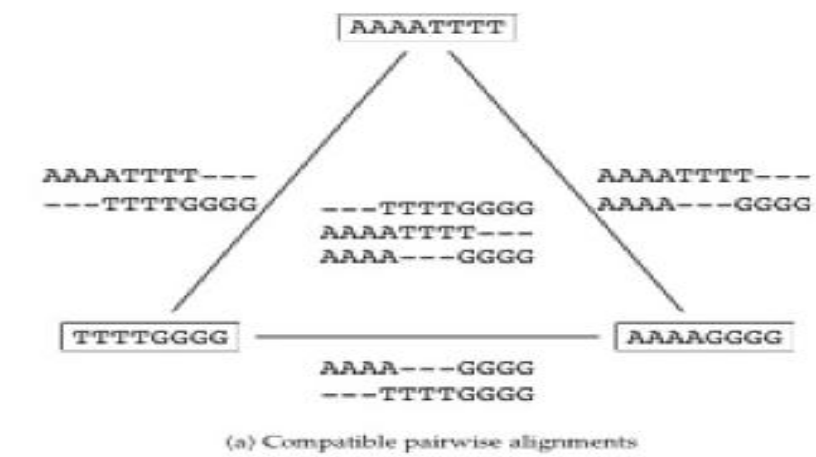
\includegraphics[width=1\textwidth]{img/simsa1.png}
		\caption{From optimal PAs to MSA.}
		\label{ex1PA}
	\end{minipage}
	\hspace{0.1cm}
	\begin{minipage}[t]{0.5\linewidth} 
		\centering
		
\includegraphics[width=1\textwidth]{img/simsa2.png}
		\caption{From optimal PAs to MSA.}
		\label{ex2PA}
	\end{minipage}        
\end{figure} 
 
Figures \ref{ex1PA} and \ref{ex2PA} show example of multiple pairwise alignments that can be combined into a single multiple-alignment, since there is no ambiguity. Instead if we consider the following example: \\

\begin{figure}[H]
	\begin{minipage}[t]{0.5\linewidth}
		\centering
		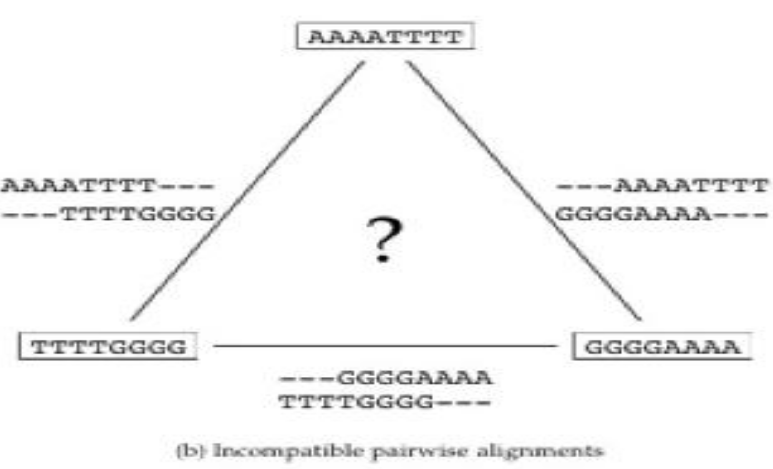
\includegraphics[width=1\textwidth]{img/nomsa1.png}
		\caption{From optimal PAs to MSA.}
		\label{ex3PA}
	\end{minipage}	
	\hspace{0.1cm}
	\begin{minipage}[t]{0.5\linewidth} 
		\centering
		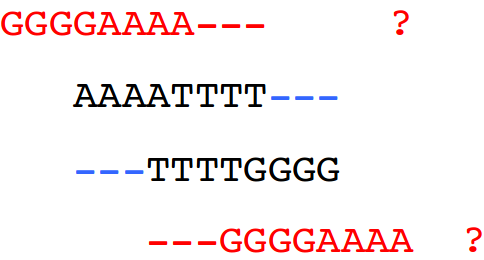
\includegraphics[width=1\textwidth]{img/nomsa2.png}
		\caption{From optimal PAs to MSA.}
		\label{ex4PA}
	\end{minipage}        
\end{figure} 
Figures \ref{ex3PA} and \ref{ex4PA} show an example of pairwise alignments that cannot be combined into a single multiple alignment since there is \textbf{ambiguity}. What we can see is that there is ambiguity because the sequence \verb|GGGGAAAA| can be either aligned on the A prefix or in the G suffix.\\

From an optimal multiple alignment we can infer pairwise alignments between all pairs of sequences, but they are not necessarily optimal. From optimal pairwise alignment between all pairs of sequences it is difficult to infer a \textbf{good multiple alignment}.
\section{Scores}
In order to get the best possible multiple alignment for MSA we introduce a score to each possible solution and we pick the best one. There exists 3 ways for computing the score:
\begin{itemize}
	\item Multiple Longest Common Subsequence score (LCS score)
	\item Entropy Score
	\item Sum of Pairs Score (SP score)
\end{itemize}
They have a common assumption: \textbf{Independence of positions.}


\paragraph{Multiple LCS score}
A column is a \textbf{match} if all the letters in the column are the same. The total score is the number of matches.
\image{img/lcs.png}{LCS Example.}{0.1}

This scoring algorithm is very good only for very similar sequences, and remember that still preserve the independence of positions.
\paragraph{Entropy score}
Define \textbf{frequencies} for the occurrence of each letter in each column of multiple alignment.

\begin{align}
\begin{bmatrix}
$A$&$A$&$A$ \\
$A$&$A$&$A$ \\
$A$&$A$&$T$ \\
$A$&$T$&$C$
\end{bmatrix}
\end{align}

\begin{itemize}
	\item $p_A = 1, p_T = p_G = p_C = 0$ ($1^{st}$ column)
	\item $p_A = 0.75, p_T = 0.25, p_G = p_C = 0$ ($2^{st}$ column)
	\item $p_A = 0.50, p_T = 0.25, p_G = 0.25, p_C = 0$ ($3^{st}$ column)
\end{itemize}
Compute \textbf{entropy} of each column:
$$- \sum_{X = A,T,G,C} p_x \times \log_2p_x$$
Example:
\begin{align}
entropy & \begin{bmatrix}
$A$ \\
$A$ \\
$A$ \\
$A$
\end{bmatrix} = 0 && \text{\textbf{Best case}}
\end{align}


\begin{align}
entropy & \begin{bmatrix}
$A$ \\
$T$ \\
$G$ \\
$C$
\end{bmatrix} = -\sum\frac{1}{4}\log_2\frac{1}{4} = 2 && \text{\textbf{Worst case}}
\end{align}
\textbf{Entropy for a multiple alignment} is the sum of entropies of its columns.
$$\sum_{\text{over all columns}}(- \sum_{X = A,T,G,C} p_x \times \log_2p_x)$$
Then the best alignment is reached minimizing this quantity.
\image{img/entropy.png}{Entropy score example.}{1}

\paragraph{Sum of Pairs} From a multiple alignment, we can infer pairwise alignments between all sequences, but they are not necessarily optimal. This is like projecting a 3D multiple alignment path onto a 2D face of the cube. In other words a 3D alignment can be projected onto a 2D plane to represent an alignment between a pair of sequences.
\image{img/projection3d.png}{All 3 Pairwise Projections of the Multiple Alignment}{0.4}

Consider pairwise alignment of sequences $a_i$ and $a_j$ imposed by a multiple alignment of $k$ sequences. Denote the score of this sub-optimal (not necessarily optimal) pairwise alignment as: $s^*(a_i,a_j)$. Sum up the pairwise score for a multiple alignment:
$$s(a_1,\dots,a_k) = \sum_{i,j} s^*(a_i,a_j) $$
It corresponds to consider more possible ancestors. In evolution, mutations are counted more than once. So, if we want to align $4$ sequences we have $6$ pairwise alignments.
Given $a_1$,$a_2$,$a_3$,$a_4$ we have:
$$s(a_1,\dots, a_4) = \sum s^*(a_i,a_j) = s^*(a_1,a_2)+s^*(a_1,a_3)+s^*(a_1,a_4)+s^*(a_2,a_3)+s^*(a_2,a_4)+s^*(a_3,a_4)$$
\image{img/sumpairsexample.png}{Sum of Pairs Score example.}{0.8}

\subsection{Representation of MSA: Profile}
\image{img/msaprofile.png}{MSA representation Example.}{0.8}
MSA representation takes in consideration:
\begin{itemize}
	\item Symbols frequencies
	\item It is an \textbf{exact and compact representation} of the multiple alignment
	\item A \textbf{threshold} can simplify the profile
	\item Useful for searching in DB
	\item We can align a sequence against a profile
	\item We can align a profile against a profile
\end{itemize}

\subsection{Aligning alignments}
Another interesting problem regards the possibility of aligning two different alignments.

\image{img/alignalignments.png}{Align alignments example.}{0.5}

A suggestion consists on considering the two profiles.

\subsection{Aligning a sequence to an alignment}
We define as $R_{ij}$ element of the score matrix (PAM/BLOSUM) and $x = x_1 \dots x_m$ sequence to be aligned. We want to align a profile $A$ with m columns.

\begin{align}
x_k \text{~is~aligned to}~~~ A_h = & \begin{bmatrix}
a_1 \\
\dots \\
a_n
\end{bmatrix}
\end{align}

\textbf{Score}(x,A) = $\sum_isc(x_i,A_i)\qquad i \in [1,m]$ with\\
\textbf{sc}($x_k, A_h$) = $\sum_ia_iR_{xki} \qquad i \in [1,21]$

\subsection{Aligning an alignment to an alignment}
We define $R_{ij}$ element of the score matrix (PAM/BLOSUM) and a profile $A$ to be aligned with another one $B$, both with m columns.

\begin{align}
B_h = & \begin{bmatrix}
b_1 \\
\dots \\
b_n
\end{bmatrix}
\end{align}

is aligned to:

\begin{align}
A_h = & \begin{bmatrix}
a_1 \\
\dots \\
a_n
\end{bmatrix}
\end{align}
\textbf{sc}$(A_h,B_k) = \sum_j\sum_ia_ib_jR_{ij} \qquad i,j \in [1,21]$\\
\textbf{score}$= \sum_k sc(A_k, B_k) \qquad k \in [1,m]$

\section{Heuristic Methods for MSA}
MSA can be solved by different heuristic methods:
\begin{itemize}
	\item Carillo-Lipman method
	\item Heuristic Greedy method
	\item Progressive Alignments (ClustalW)
	\item Iterative Alignments (Deterministic and Stochastic)
	\item Partial Order Alignments (POA)
\end{itemize}

\subsection{Carillo-Lipman}
One of the heuristic algorithms for MSA is the \textbf{Carillo-Lipman Bound procedure}(1988). It computes a polyhedron around the diagonal in a hypercube. This bounds the search space for finding MSA. It computes the optimal alignment scores only in the grey volume. 
\image{img/carillo.png}{Carillo-Lipman space.}{0.3}
The grey volume is computed on the one side by the optimal alignments found for each pair of sequences, and on the other by a heuristic multiple alignment of the 3 sequences.\\

\paragraph{Procedure.} The method can be easily described with the following steps:
\begin{itemize}
	\item Consider the pairwise alignments of each pair of sequences and create a phylogenetic tree from these scores.
	\item produce a draft MSA built from the phylogenetic tree.
	\item the pairwise alignments and draft MSA provide a \textbf{reduced solution space} on which dynamic programming is used to find the solution.
\end{itemize}

\paragraph{Properties.} This methods does not guarantee an optimal alignment for all the sequences because most of the solution space is excluded from search. It is useful when at most 8 sequences of average size and similarity need to be aligned.

\subsection{Heuristic Greedy Approach}
The algorithm works:\\ 
"\textit{Choose most similar pair of strings and combine them into a profile, thereby reducing alignment of k sequences to an alignment of $k-1$ sequences/profiles. Repeat.}"\\

This is a heuristic greedy method that can be applied both to sequences and to profiles.

\image{img/heuristicGreedy.png}{Heuristic Greedy Method.}{0.7}
Consider these $4$ sequences:
\image{img/heuristicExample.png}{Sequences Example.}{0.3}
with scores: match = 1, mismatch = -1 and gap = -1.

\image{img/heuristicSolvedExample.png}{Solution for heuristic example procedure(1).}{0.7}

\image{img/heuristicExampleSolved2.png}{Solution for heuristic example procedure(2).}{0.6}

\subsection{Progressive Alignments (ClustalW)}
Progressive alignment is a variation of the greedy algorithm with a somewhat more intelligent strategy for choosing the order of alignments. It is based on the idea of building a phylogenetic tree out of the sequences, the tree is used to decide which sequences are aligned first, because of their similarity. We can find different algorithms like: CLUSTAL, T-COFFEE.

\paragraph{ClustalW}
Popular MSA tool based on progressive alignment. $W$ stands for \textit{weighted} since different parts of alignment can be weighted differently. The weights may depend by the sequences relations or by being over or under-estimated: Three-step process:
\begin{enumerate}
	\item Construct pairwise alignments.
	\item Build guide tree.
	\item Progressive alignments guided by the tree.
\end{enumerate}
Different score matrices can be used depending on sequences relations. Gaps are permanent and it can use profiles to compare sequences.\\

Algorithm definition:
\begin{enumerate}
	\item Align each sequence $v_i$ against each other $v_j$ giving a \textbf{similarity matrix}. Similarity is measured counting the ration between exact matches and sequence length. $$\text{similarity} = \frac{\text{exact matches}}{\text{sequence length}}$$ 
	\image{img/step1.png}{ClustalW step 1.}{0.5}
	
	\item Create \textbf{guide tree}, which roughly reflect evolutionary relations, using the similarity matrix. ClustalW uses the neighbor-joining method.
	\image{img/step2.png}{ClustalW step 2.}{0.5}
	
	\item Start by aligning two most similar sequences. Following the guide tree, add the next sequences, aligning them to the existing alignment.
	\image{img/step3.png}{ClustalW step 3.}{0.7}
	\image{img/step3_2.png}{ClustalW step 3 example.}{0.9}
	\begin{itemize}
		\item \textbf{*} identical.
		\item \textbf{:} conserved substitution (same group).
		\item \textbf{.} semi-conserved subdivision (similar shapes).
	\end{itemize}
\end{enumerate}

\paragraph{Properties}
Progressive alignment is the most widely used method. It has some advantages:
\begin{itemize}
	\item \textbf{Speed}
	\item \textbf{Simplicity}
	\item A reasonable \textbf{Sensitivity}
\end{itemize}
But it has also some disadvantages:
\begin{itemize}
	\item It is an \textbf{heuristic method}
	\item It is \textbf{highly sensitive} to the choice of initial aligned pairs
	\item The initial pairs are \textbf{frozen} even if subsequent steps show that they are not correct
	\item The likelihood of large errors in the initial alignments increases as the sequences become more distantly related, hence they work well for close sequences, but they \textbf{deteriorate for distance sequences}.
\end{itemize}

\subsection{Iterative Alignments - Deterministic}
Progressive alignment results can be sensitive to inaccuracies in the initial pairwise alignments. Iterative methods produce an initial global alignment (i.e. obtained by a progressive method) and then iteratively refine it in order to \textbf{optimize an objective function}. The algorithm works as follow:
\image{img/iterative.png}{Iterative alignments procedure.}{1}
The procedure is guaranteed to \textbf{converge to a local maximum}. If the initial alignment is poor, it may not converge to the global maximum. Examples of deterministic iterative approaches are: PRRP, DIALIGN, etc...

\subsection{Iterative Alignments - Stochastic}
\begin{itemize}
	\item \textbf{Genetic Algorithm:}
	\begin{itemize}
		\item Randomly generate MSA (generations)
		\item Alignments die or survive depending on their fitness (score)
		\item Mutations rearrange them with the introduction of gaps at varying positions or recombine them.	
		\item An objective function is optimized.
	\end{itemize} 

	\item \textbf{Simulated Annealing:}
	\begin{itemize}
		\item An alignment is randomly modified
		\item Its score is assessed
		\item according to an acceptance function it is kept or discarted.
		\item The acceptance function becomes more stringent at each iteration.
	\end{itemize} 
	\item \textbf{Hidden Markov Models}
	\item \textbf{Not ab initio!}
\end{itemize}

\subsection{Partial Order Multiple Alignment (POA)}
Multidomain proteins evolve not only through point mutations but also though \textbf{domain duplications} and \textbf{domain re-combinations}. Often impossible to align all protein sequences throughout their entire length.
\image{img/alignmedGraph.png}{Alignmed as a Graph.}{0.95}
\image{img/pathgraph.png}{Representing sequences as paths in a graph.}{0.95}

Partial Order Multiple Alignment has two goals:
\begin{itemize}
	\item Finding a graph that represents a domain structure (model).
	\item Finding mapping of each sequence to this graph.
\end{itemize}
The solution consists on using the PO-MSA algorithm, which basically construct a graph G such that every sequence in the set of sequences S is a path in G. \\
The POA algorithm aligns sequences onto a directed acyclic graph (DAG):
\begin{itemize}
	\item Guide Tree Construction
	\item Progressive Alignment Following Guide Tree
	\item Dynamic Programming Algorithm to align two PO-MSAs (PO-PO Alignment).
\end{itemize}
Alignments of graphs is done using the dynamic programming definition:

$$S(n,o) = \text{max}_{p\rightarrow n, q \rightarrow o} \begin{cases}
S(p,q) + s(n,o) & \\
S(p,o) + \Delta(n) & \text{n: node in G}\\
S(n,q) + \Delta(o) & \text{o: node in G}^\prime
\end{cases}$$
Then value $S(n,o)$ represents the score assigned to the alignment, with $s(n,o)$ as the cost of match or mismatch between node n and o, and with $\Delta(n)$, $\Delta(o)$ as the costs for deleting node n or node o from the alignment.

\section{Multiple Alignments Remarks}
For MSA there is no satisfactory theory, improvements driven by results, not by the theory. For that reason importance of visualization tools can be important for the evaluation and inspection. In particular we have two types of representations:
\begin{itemize}
	\item \textbf{Visualization (ClustalX)} 
	\image{img/clustalx.png}{Visualization of MSA.}{0.85}
	
	\item \textbf{Visualization: sequence logo}
	\image{img/logo.png}{Visualization: sequence logo}{0.8}
	 A sequence logo shows the more conserved residues as larger characters, the total height of a column is proportional to how conserved that position is.

\end{itemize}

\chapter{Genome Sequencing}
Genome sequencing is the process of determining a certain part or the complete DNA sequence of an organism's genome at a single time. Old biological techniques, that took into consideration small fragments of DNA for automatically sequencing, were not based on computation:
\begin{itemize}
	\item \textbf{Sanger sequencing} (\textit{Chain-Termination Method}): single stranded DNA molecules that differ in length by one nucleotide can be separated by polyacrylamide gel electrophoresis. Length ranging from 10 to 1500 nucleotides and the sequence can be read on the gel.
	\image{img/Sanger}{Sanger Technique.}{0.57}
	\item \textbf{PCR} (\textit{Polymerase Chain Reaction}).
	\image{img/PCR}{PCR Technique.}{0.9}
\end{itemize}

Sequencing a genome has an intrinsic complexity, for example, it is necessary to consider the degree of reliability of the obtained sequence. Repeated regions are mostly problematic, indeed, genomes may contain a lot of repeated sequences, for instance, in the Homo Sapiens genome, the repeated regions represent around the 35-50 \% of the total genome. For this reason, important questions are: Does the genome under the examination present repeated regions? What kind of repetitions? How long are these regions? What is the "degree of conservation" of the repeated regions?\\
When we talk about genome sequencing techniques, surely, we must consider the \textbf{shotgun sequencing} technique and its main variant the \textbf{double-barreled shotgun}. All sequencing projects consists in the following phases. After fragmenting and amplifying the DNA, for any DNA sequence obtained:
\begin{enumerate}
	\item DNA sequencing. (Biologist)
	\item Fragment-assembly. (Computer Scientist)
	\item Finishing. (Biologist)
\end{enumerate}

\section{Shotgun Sequencing}
Shotgun was developed in 1982 by Sanger and successively refined. It has three phases as can be seen in the following lines.
\subsection{Step 1 - DNA sequencing.}
It starts partitioning the DNA into sequences, suppose a length of 100.000 bp (\textit{base pairs}), and for each one apply the following steps:
\begin{enumerate}
	\item Produce a large number of copies of the source DNA (\textit{amplification}).
	\item Random fracture the sample, either using sound (\textit{sonication}) or passing it through a nozzle under pressure (\textit{nebulation}). The process produces a uniformly random partitioning of each copy of the source sequence into a collection of \textbf{DNA fragments}.
	\item Fragments that are too large or too small are removed, using gel electrophoresis. The band of gel containing the desired size is selected.
	\item The size-selected fragments are inserted in the DNA of genetically engineered bacterial virus (\textit{phage}), called \textbf{vectors}. Usually, one fragment is inserted into a vector at a predetermined point, called \textbf{cloning site}. The fragments are called \textbf{inserts} and the collection of fragments is called a \textbf{shotgun library}.
	\item A bacterium is infected with a single vector, which reproduces itself producing a bacterial colony containing million of copies (clones) of the vector and its associated insert. This procedure is repeated simultaneously for as many inserts as desired.
	\item By design, the vector permits a sequencing reaction (Sanger - chain termination method) to be performed, starting just at the fragment's insertion point. The sequencing reaction produces a read of the first 300-900 bases of one end of the insert.
\end{enumerate}
With these steps, a set of reads, randomly sampled from the source sequence is produced.
\image{img/DNAsequencing}{DNA Sequencing.}{0.8}
\paragraph*{Failure points: Bias.} A failure in the process may occur if the reads are not randomly sampled but biased to come from particular regions of the source DNA. This can happen for three reasons:
\begin{enumerate}
	\item The fracturing of the sample might be biased.
	\item The insertion of fragments into vectors might be biased.
	\item Some insert/vector combinations might not clone properly because the insert has reacted toxically with the host/vector environment.
\end{enumerate}
Practical evidence suggests that the first two biases are minimal in well-performed experiments, but the third bias definitely exists. Picking host/vector combinations for which the insert DNA will be relatively inert will reduce the toxicity bias.

\paragraph*{Failure points: Errors in reads.} Reads may contain errors for a variety of reasons: 
\begin{itemize}
	\item Technicians must screen the failed reads from vectors where no insert occurred.
	\item The sequencing reaction begins at one end of the insert location or at the other. The initial part of a read contain the vector sequence leading up to the beginning of the insert. This bit of vector sequence must be carefully removed.
	\item If an insert is short, technicians might need to trim the vector sequence from the end of a read.
\end{itemize}  

\subsection{Phase 2 - Fragment assembly}
Once all the reads of the shotgun library are available, the computational problem starts: it is necessary to arrange all the fragments to obtain the source DNA sequence. This is called \textbf{fragment-assembly problem}.
\image{img/fragmentAssembly}{Fragment-Assembly step.}{0.8}

\paragraph*{Redundancy and coverage.} The Number of sequenced (read) bases must be sufficiently high to ensure that all the genome has been covered. Now, it is important understand the meaning of some specific information that will be useful in the following pages:
\begin{itemize}
	\item \textbf{G:} length of the target sequence (genome size).
	\item \textbf{\textbf{F} = $\{f_1, f_2, \dots, f_R\}$:} set of reads.
	\item \textbf{L:} average length of a read.
	\item \textbf{R:} number of reads in shotgun dataset.
	\item \textbf{N = RL:} total number of base pairs sequenced.
\end{itemize}
The \textbf{average redundancy} or \textbf{coverage} is given by:
$$c = N/G ~ = ~ \text{number of sequenced bases}/\text{genome size}$$
For example suppose that 4 million bases of a bacterial genome have been sequenced and that the genome size is 4 Mb, then the coverage is 1x.\\
As genome coverage grows, the closure of regions not yet sequenced becomes highly probable. By using the Poisson distribution equation, it is possible to establish the probability $P_0$ that a base has not been sequenced, with respect to the coverage value $c$:
$$P_0 = e^{-c}$$
The percentage of effective coverage is:
$$\% Cov = 100 \cdot (1-e^{-c})$$
	\begin{figure}[H]
	\begin{minipage}[t]{0.45\linewidth}
		\centering
		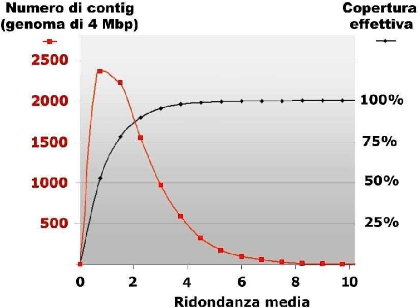
\includegraphics[width=\textwidth]{img/coverage}
		\caption{Coverage function.}
	\end{minipage}
	\hspace{1.8cm}
	\begin{minipage}[t]{0.42\linewidth} 
		\centering
		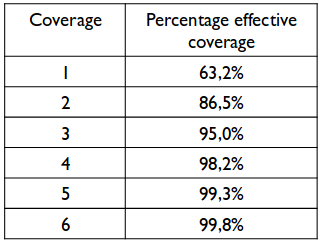
\includegraphics[width=\textwidth]{img/coverage_table}
		\caption{Percentage effective coverage.}
	\end{minipage}        
\end{figure}
\FloatBarrier
Usually a coverage of 10 is considered.

\paragraph*{Data peculiarities: bias and errors.} A computational solution of the fragment-assembly problem must consider the following data characteristics:
\begin{itemize}
	\item \textbf{Incomplete coverage:} not every bp of the sequence under examination is sequenced exactly $c$ times because of the stochastic nature of the process. The random steps might be biased and some parts of the sequence can be covered more than $c$ times, while other parts aren't covered at all.
	\item \textbf{Gaps:} are contiguous regions of maximal length that are not covered. Gaps lead to fragmented or incomplete solutions of the problem.
	\item \textbf{Sequencing errors:} the sequencing process of the inserts can cause errors which depend on the position in the insert ($<1\%$ for the first 500 bases; up to $15\%$ from 600 to 900 bases). Quality values can be associated to the bases in the reads. 
\end{itemize}

\paragraph*{Data peculiarities: orientation and repeats.} Other data features can be:
\begin{itemize}
	\item \textbf{Orientation:} the DNA is a double string. Only one end of the insert is sequenced. The right sequence to use might be either the read or its reversed 
	complement. Usually solved by sequencers.
	\item \textbf{Repeated sequences:} can cause assembly errors. In the picture the top represents the correct layout of three DNA sequences. The bottom shows a repeat collapsed in a misassembly.
\end{itemize}
\image{img/pec_orientation}{Repeated sequences.}{0.6}

\par \bigskip \noindent
Several computer science solutions are available when we consider the fragment-assembly steps:
\begin{itemize}
	\item \textbf{Exact approach:} \textit{shortest superstring problem} (SSP)
	\item \textbf{Heuristic (and greedy) approach:} \textit{Overlap-Layout-Consensus} (OLC), where:
	\begin{itemize}
		\item \textbf{Phase 1: overlap detection} (\textit{without errors}) $\rightarrow$ all pairs suffix-prefix matching.
		\item \textbf{Phase 1: overlap detection} (\textit{with errors}) $\rightarrow$ we can have also imperfect suffixes or prefixes composed by gaps/mismatches (\textit{semi-global alignment}) or matches that are not exactly suffixes or prefixes (\textit{LCS}). It has several implementations as: 
		\begin{itemize}
			\item \textbf{Semi-global alignment} (\textit{exact}): it is exact since it keeps only prefixes and suffixes but it can contain errors since there can be the presence of mismatches and gaps.
			\item \textbf{LCS}: Longest Common Substring problem (\textit{heuristic}). It keeps the longest common substring between two strings but this doesn't ensure the fact that the string is a suffix or a prefix, it could be also on the central part of the string.
			\item FASTA or BLAST (\textit{heuristic}).
		\end{itemize}
		\item \textbf{Phase 2: Fragment Layout} $\rightarrow$ a greedy approach.
		\item \textbf{Phase 3: Consensus} $\rightarrow$ by using multiple sequence analysis.
		\item \textbf{Graph-based OLC}
	\end{itemize}
\end{itemize}

\subsubsection{SSP - An exact approach}
A first approach is to formalize the problem in terms of a string problem, more precisely, the \textbf{shortest superstring problem} (\textit{SSP}). Given a set of strings $P=\{s_1, s_2, \dots, s_k\}$, a superstring of P is a single string that contains every string in P as a substring, for example, a concatenation of the strings of P in any order produces a superstring.\\
Given $P =\{\verb|abcc|, \verb|efab|, \verb|bccla| \}$ then "$\verb|bcclabccefab|$" and "$\verb|efabccla|$" are two superstrings of P. Moreover "$\verb|efabccla|$" is a shortest superstring.\\
Looking for the shortest superstring of P, strings in P are the reads and the shortest superstring containing all the strings in P is a good candidate for target DNA (parsimony assumption).\\
SSP has problem with repeats as can be seen in the following example considering the following sequence:
$$\verb|AATCTGGAGCTCT|$$
and its fragments:
\begin{enumerate}
	\item $\verb|AAT|$
	\item $\verb|CTGG|$
	\item $\verb|AGC|$
	\item $\verb|TCT|$
\end{enumerate}
The sequence can be obtained by simply concatenating the four fragments. However, the shortest substring of the set of fragments is:
$$\verb|AATCTGGAGC|$$
that collapses the repeated string "$\verb|TCT|$". The shortest substring problem is applied to fragment-assembly and data compression, it is an NP-Hard. For this reason heuristics to solve the SSP problem may be used, there are, indeed, polynomial algorithms which approximate the optimal solution of SSP within an arbitrary but predetermined constant.
Besides this, SSP have further problems in modeling the fragment-assembly such as:
\begin{enumerate}
	\item \textbf{SSP does not model possible read errors}. Errors might include:
	\begin{itemize}
		\item Insertion errors where a base is wrongly present in a fragment.
		\item Deletion errors where a base is absent from a fragment.
		\item Substitution errors where a base is substituted for another in a fragment. \item Chimeric errors where two disjoint fragments join to from a single non-existing fragment.
	\end{itemize}
	\item \textbf{SSP does not model fragment orientation}.
	\item \textbf{SSP fails in the presence of repeats}.
\end{enumerate}
For these reasons SSP is considered only of theoretical interest.

\subsubsection{OLC - An approximated approach}
OLC (Overlap-Layout-Consensus) is an approximate (heuristic) and greedy solution to the fragment-assembly problem, it consists of a three steps process:
\begin{itemize}
	\item Step 1: Overlap detection.
	\item Step 2: Fragment Layout.
	\item Step 3: Deciding the Consensus.
\end{itemize}

\paragraph*{OLC Step 1: Overlap detection (\textit{without errors}).} The problem consists of determining, for every ordered pair of reads, how much of the suffix of the first coincides with the prefix of the second. It should also consider their orientation.\\
In this specific case, without errors, for every ordered pair of strings $S_1$ and $S_2$, find the longest suffix of $S_1$ which is also a prefix of $S_2$ (\textit{suffix-prefix match problem}). Given two strings $S_1$ and $S_2$, any suffix of $S_1$ that matches a prefix of $S_2$ is called \textbf{suffix-prefix} of $S_1$ and $S_2$.
\begin{center}
	
\includegraphics[width=0.25\columnwidth]{img/OLC_1a}
\end{center}
Given a collection of strings $S=\{S_1, \dots, S_k\}$ of total length $m$, the all-pairs suffix-prefix problem is the problem of finding, for each ordered pair $S_i$ and $S_j$ in S, the longest suffix-prefix match of $S_i$ and $S_j$. The number of matches that will be done in order to retrieve the longest suffix-prefix is $k^2$.\\
An exact algorithm is based on the use of a \textbf{generalized suffix tree}. In a suffix tree a terminal edge is labelled with a string termination symbol (usually $\textdollar_i$). The algorithm consists of the following steps:
\begin{enumerate}
	\item Construct the generalized suffix-tree $T(S)$ for the $k$ strings of S (each one with its additional terminal symbol).
	\item Construct a list $L(v)$ for each internal node $v$. $L(v)$ contains index $i$ if and only if $v$ is incident with a terminal edge labelled \$$_i$ (the path-label of $v$ is a suffix of $S_i$). The list $L(v)$, for each internal node $v$, can be built in linear time during (or after) the construction of $T(S)$. Let us consider the path going from the root to the leaf $j$ representing the entire string $S_j$, the key observation is the following:
	\begin{itemize}
		\item If $v$ is a node on the path and index $i$ is in $L(v)$, then the path-label of $v$ is a suffix of $S_i$ that matches a prefix of $S_j$.
		\item So, for each index $i$, the deepest node $v$ on the path to leaf $j$ such that $i \in L(v)$ identifies the longest match between a suffix of $S_i$ and a prefix of $S_j$. The path-label of $v$ is the longest suffix-prefix match of $S_i$ and $S_j$.
		\item By one traversal from the root to leaf $j$, we can find the deepest nodes for all $1 \leq i \leq k~(i \neq j)$.
	\end{itemize}
	\item Collect all the suffix-prefix matches by traversing $T(S)$ in a depth-first manner and maintaining $k$ stacks (one for each string):
	\begin{itemize}
		\item When a node $v$ is reached, push $v$ onto the $i$-th stack, for each $i \in L(v)$.
		\item When a leaf representing the whole string $S_i$ is reached, scan the $k$ stacks and record, for each index $i$ the current top of the $i$-th stack. If the $i$-th stack is empty, then there's no overlap between $S_i$ and $S_j$.
		\item When the depth-first traversal backs up past node $v$, pop the top of each stack whose index is in $L(v)$.
	\end{itemize}
\end{enumerate}
All the $k^2$ longest suffix-prefix matches of S can be found in $O(m+k^2)$ time. Since $m$ is the size of the input and $k^2$ is the size of the output, the algorithm is time optimal. Note that:
\begin{itemize}
	\item $m$ = average read length $\times$ number of reads = $LR$
	\item $k$ = number of reads = $R$
\end{itemize}
Hence, $O(m+k^2) = O(L \cdot R + R^2)$ 

\paragraph*{OLC Step 1: Overlap detection (\textit{with errors}).} The all-pair suffix-prefix matching solve the problem under the hypothesis that the sequenced data have no errors, but \textbf{sequencing errors exist}. For this reason, the suffix-prefix matching must admit approximations. The problem is to find a suffix $S_1$ and a prefix $S_2$ whose similarity is maximum over all suffix-prefix pairs of $S_1$ and $S_2$.\\
First of all, it is important to define the concept of similarity:
\begin{itemize}
	\item Positive matches make a positive contribution to the objective function.
	\item Mismatches and gaps make a negative contribution.
\end{itemize}
The most useful weights and penalties must be fixed. From another point of view, it can be seen as a \textbf{semi-global alignment} problem, indeed, a \textbf{variant of the Needleman-Wunsch} global alignment algorithm is considered (optimal alignment by admitting initial and final gaps without penalties).\\
Given two strings $x$ and $y$ of length $n$ and $m$, the inductive definition is:
\image{img/NW-OLC}{A variant of the NW algorithm}{0.7}
The maximum score is on the last row and/or column and the aligned string can be found by following the backward pointers until one element of the first row or column is reached.\\
For example, consider the Nucleotide similarity score matrix:
\image{img/similarity_score_matrix}{Similarity score matrix}{0.25}
and fix the gap penalty $d=2$.\\
By using the given recursive equation, we want to apply the algorithm to the strings:
\begin{enumerate}
	\item $x = \verb|GCCATCT|$
	\item $y = \verb|TCTAAGC|$
\end{enumerate}
The resulting table is:
\image{img/example_table}{Example of the variant of N-W algorithm.}{0.7}
If we take into consideration the complexity of this algorithm, we know that N-W algorithm is $\theta(nm)$, considering $n \simeq m$ and equal to $L$ (average length of a read), the complexity can be indicated as $\theta(L^2)$.\\
Let $R$ be the total number of reads, then the complexity of the overlap detection phase is $\theta(R^2L^2)$. Usually $L=400\text{ or }500$ and the number of reads $R$ is very high. Hence, the overlap detection is computationally very expensive and creates a bottleneck for the fragment-assembly problem, then, instead of an exact solution, heuristic solutions can be adopted. Heuristics for overlap detection try to find ordered pairs of strings with large similarity, for instance, two strings having a sufficiently long common substring are probably overlapping substrings. The corresponding computational problem is the \textbf{longest common substring} problem (\textit{LCS}), that can be efficiently solved using a generalized suffix tree.

\paragraph*{Longest Common Substring (LCS).} This algorithm is related to the problem that starting from two strings $S_1$ and $S_2$, it is needed to find the longest common substring. An exact solution is based on the construction of the generalized suffix-tree of $S_1$ and $S_2$ in which:
\begin{itemize}
	\item The leafs represent a suffix of $S_1$ or $S_2$.
	\item Each internal node $v$ is marked with 1 and/or 2 if and only if there is a leaf in the subtree of root $v$ that is a suffix of $S_1$ and/or $S_2$.
	\item Internal nodes marked both 1 and 2 correspond to common substrings of $S_1$ and $S_2$. The longest of such substrings is the solution to the problem.
\end{itemize}
The algorithm must find the node which is marked 1 and 2 and with the \textbf{greater string-depth} (number of characters in the path from the root to the node). The algorithm steps are the following:
\begin{enumerate}
	\item Build the generalized suffix-tree for $S_1$ and $S_2$.
	\item Mark the internal nodes and compute their string-depth.
	\item Return the substring with maximal string-depth which corresponds to a node marked both 1 and 2.
\end{enumerate}
The first step requires linear time with respect to the sum of the lengths of $S_1$ and $S_2$, also the further steps can be performed in linear time by tree traversal.\\
The LCS problem is only an heuristic for the overlap detection phase and for this reason it could not bring us to an optimal solution. For example:
\begin{center}
	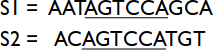
\includegraphics[width=0.22\columnwidth]{img/LCS_example}
\end{center}
The longest common substring is underlined but we can suppose the fact that it could be a repeat, then the two strings may not be overlapping or the fact that this procedure doesn't allow for errors.

\paragraph*{Further Heuristics.} Other heuristics use BLAST or FASTA to find a good local alignment among all possible pairs of strings. The higher the score, the greater the probability that the two corresponding strings are overlapping.\\
These techniques greatly reduce the overall computation time for sequence-assembly. They allow for errors in the reads.

\paragraph*{OLC Step 2: Fragment Layout - Greedy solution.} In this phase one tries to rebuild the target DNA sequence by using the overlaps. There are various approaches to this problem. The first (and most practical) implementations follow some variant of the following greedy approach:
\begin{itemize}
	\item The string pair with highest suffix-prefix (or overlapping) score is chosen and merged. This step forms the \textbf{first contig} (set of contiguous DNA segments):
	\begin{center}
		
\includegraphics[width=0.22\columnwidth]{img/contigA}
	\end{center}
	\item Then, the next highest score pair is selected and merged, resulting either in one contig containing three strings (\textit{b}) or in two separate contigs containing four strings (\textit{c}):
	\begin{center}
		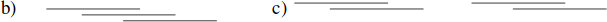
\includegraphics[width=0.8\columnwidth]{img/contigBC}
	\end{center}
	\item Iterate. 
\end{itemize} 
Since the suffix-prefix overlaps are determined by similarity criteria, gaps are allowed in the suffix-prefix matches. As successive inserts are added into a contig, additional gaps may have to be inserted into the added string to be consistent with gaps in the previously inserted strings.\\
The main difficulty in this phase is to decide whether two fragments with a good overlapping score:
\begin{itemize}
	\item \textbf{Do effectively overlap} (hence their differences are due to sequencing errors).
	\item Or \textbf{represent a repeat} in the genome (hence their differences are due to mutations).
\end{itemize}

\paragraph*{OLC Step 3: Consensus.} In this phase we must determine the consensus on each contig. For each position of a contig it may happen that:
\begin{itemize}
	\item All characters coincide: no problem for that position.
	\item There is a disagreement in the aligned characters in that position: a choice has to be made.
\end{itemize}
Various approaches to obtain the consensus sequence:
\begin{itemize}
	\item The simplest one reports the frequency of each character at each position (\textit{profile}) and let the user decide how to use that information.
	\item Alternatively a consensus sequence can be obtained by taking the plurality of characters on each position, provided the plurality is above some preset threshold.
\end{itemize}

\paragraph*{OLC: A general overview.} The OLC assemblers discussed so far are called \textbf{greedy assemblers} because they employ greedy algorithms in the layout phase. The greedy algorithms apply one basic operation: given any read or contig, add one more read or contig, this basic operation is repeated until no more operations are possible. Each operation uses the next highest-scoring overlap to make the next join. The scoring function measures, for instance, the number of matching bases in the overlap, thus the contigs grow by greedy extension, always taking on the read that is found by following the highest-scoring overlap.\\
However, greedy assemblers have also the following problems:
\begin{enumerate}
	\item The greedy algorithms can get stuck at \textbf{local maxima}.
	\item Overlaps induced by repetitive sequences may score higher than real overlaps.
	\item The greedy algorithms need mechanisms to avoid incorporating false-positive overlaps into contigs.
	\item An assembler that builds on false-positive overlaps will join unrelated sequences and produce \textbf{chimera}.
\end{enumerate}

\paragraph*{Graph-based OLC.} OLC assemblers can be also graph-based, they use the so-called \textbf{overlap graph}. An overlap graph represents the reads and their overlaps:
\begin{itemize}
	\item Nodes represent the reads.
	\item Edges represent overlaps.
\end{itemize}
The graph-based OLC approach consists of three phases:
\begin{enumerate}
	\item \textbf{Overlap:} overlap detection using one of the already discussed techniques.
	\item \textbf{Layout:} construction and manipulation of an overlap graph, paths in the graphs are potential contigs. The overlap graph does not represent single bases, so large-genome graphs may fit into computer memory.
	\item \textbf{Consensus:} a multiple sequence alignment (MSA) determines the layout and then the consensus sequence. Heuristics are generally used for MSA. The consensus phase must load the sequences of bases into memory.
\end{enumerate}
For instance, suppose to have three copies of an unknown target DNA sequence:
\begin{center}
	
\includegraphics[width=0.8\columnwidth]{img/example_graphOLC}
\end{center}
Suppose the obtained reads are: \verb|accgt|, \verb|aggt|, \verb|acgatac|, \verb|accttta|, \verb|tttaac|, \verb|gataca|, \verb|accgtacc|, \verb|ggt|, \verb|acaggt|, \verb|taacgat|, \verb|accg|,\verb|tacctt|.
\begin{itemize}
	\item The first step is the overlap detection among reads.
	\item The second step is the construction of a graph whose nodes represent reads and edges indicate overlaps between reads.
	\image{img/OLC_exampleGraph}{Example of a graph-based OLC.}{0.65}
	\item The third step consists in refining the graph by detecting the transitive edges and solving the ambiguities. The output of this step is a set of simple paths with no intersections, each one corresponding to a contig. The consensus sequence is obtained by performing a multiple alignment (MSA) of the reads which compose the path under examination.\\
	In our example we obtain a single path: \verb|accgtacctttaacgatacaggt|. This is a very simple case in which no errors, no repetitions and a little coverage is present.
\end{itemize}



\subsection{Phase 3 - Finishing}
Imperfect coverage, repeats, and sequencing errors cause the assembler to produce not one, but hundreds or even thousands of contigs. The task of closing gaps between contigs and obtaining one complete sequence is called \textbf{finishing}.
\image{img/finishing}{Finishing procedure.}{0.8}
A process called \textbf{scaffolding} is used to order and orient the contigs with respect to each other into larger structures called \textbf{scaffolds}. A scaffold is a maximally linked and ordered set of contigs.\\
In this phase it is possible to distinguish two types of gaps:
\begin{itemize}
	\item The gaps between contigs belonging to the same scaffold are called \textbf{sequence gaps}. They represent genuine gaps in the sequence.
	\item The gaps between scaffolds are called \textbf{physical gaps} because the physical DNA that would span them is either not present in the clone inserts or indeterminable due to misassemblies. Filling these gaps is more difficult and it involves a large amount of manual labor and complex laboratory techniques. 
\end{itemize}

\section{Double-barreled shotgun sequencing}
It is a main variant of the shotgun sequencing: the inserts average length, $l$, is longer than $2L$ and both ends of the insert are sequenced.\\
This procedure gives rise to a pair of reads, called \textbf{mates}, that are in opposite orientation and at a distance from each other approximately equal to $l$ (the insert average length).\\
The main difference with the shotgun sequencing is the fact that in this case we take into consideration information that are both in the left and the right bound. In this way it is possible to reconstruct the sequence from both sides.
\image{img/doubleShotgun}{Double-barreled shotgun sequencing schema.}{0.8}
Once contigs are built, they must be oriented and joined and clone mate information is relevant for this.
\image{img/doubleShotgun2}{Mates are useful for scaffolding.}{0.8}
A \textbf{scaffold} is a maximally linked and ordered set of contigs.
\image{img/doubleShotgun3}{Scaffolding: contigs order.}{0.7}
The mate pairing information can be used for:
\begin{itemize}
	\item \textbf{Ordering contigs:}
		\begin{enumerate}
			\item If a read in a contig has its mate in another contig, then we can suppose (by knowing the average length $l$ of the inserts) that the two contigs are adjacent.
			\item There should be various mate pairs in two possibly adjacent contigs, if their number (coverage) gives sufficient support, we can order contigs with a good reliability.
		\end{enumerate}
	\item \textbf{Identifying repeats:} the probability that both reads of an insert fall into the same repeat is low. This depend on $l$ and on the size of the repeat.
\end{itemize}
In order to build a scaffold, it is essential to create a graph whose nodes are contigs and an edge links two nodes when mate pairs bridge the gap. This lead to have computational problems as finding all the connected components in the graph, finding a consistent orientation for all nodes and embedding the graph in a sequence respecting estimates on edge lengths.\\
\textbf{Sequence gaps} are gaps in the clone which can be resequenced by PCR. \textbf{Physical gaps} are, instead, gaps between scaffolds. They corresponds to parts of DNA not present in the clones (not in the library). Mates can be used also to distinguish the two cases. 
\image{img/doubleShotgun4}{Scaffolding gaps.}{0.7}

\section{Techniques used for sequencing human genome}
Three different strategies have been used for sequencing the human genome:
\begin{itemize}
	\item Hierarchical sequencing used by HGP. This method is also called clone-by-clone sequencing or BAC-by-BAC sequencing.
	\item Sequence-tagged connector approach (\textit{a variant of hierarchical sequencing})
	\item Whole-genome shotgun sequencing used by Celera Genomics.
\end{itemize}

\subsection{Hierarchical sequencing}
The hierarchical sequencing approach can be sum up with the help of the following image:
\image{img/hierarchical}{Hierarchical sequencing.}{0.7}
The algorithm is subdivided in the following steps:
\begin{enumerate}
	\item Creation of a BAC library: random fragmentation of the genome into sequences of 50-300 kbp length, then inserted into BACs (Bacterial Artificial Chromosomes).
	\item Determining an assembly or \textbf{physical map}.
		\begin{center}
			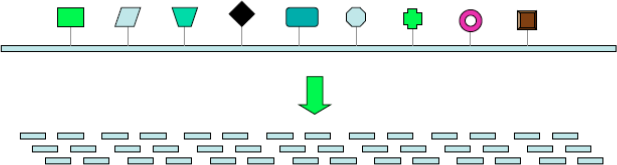
\includegraphics[width=0.8\columnwidth]{img/hierarchical3}
		\end{center}
		A map of the genome may be useful to order the fragments. A physical map is given by a set of markers (often genes or known patterns, such as enzymes or specific proteins) in the genome. The metric used is based on observable or countable physical features, usually the number of nucleotides between two points. The physical map must be accurate: error in this phase could produce "chimera" chromosomes.
	\item Determining a minimal tiling path of BACs that covers the genome, that is a set of clones with minimal overlapping. Overlaps between BAC inserts are determined on the basis of fingerprint data on each insert.
	\item Shotgun sequencing of each tiling clone.
	\item Finishing phase.
		\begin{center}
			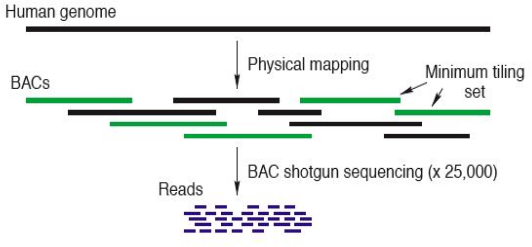
\includegraphics[width=0.8\columnwidth]{img/hierarchical2}
		\end{center}
\end{enumerate}
The clone-by-clone technique requires two separates processes: \textbf{sequencing} and \textbf{physical mapping}. The first one is heavily automated, while the second one requires a lot of hand working.\\
Physical maps are difficult and time consuming to build, on the other hand, they are useful for studying specific genome sectors and allow for a scalable approach. Moreover they ease the finishing phase.

\subsection{Sequenced-tagged connector approach}
A variant of the hierarchical approach which avoids the building of a physical map. It consists on the following steps:
\begin{enumerate}
	\item A library BACs is sequenced (600.000 for the human genome).
	\item A set of seed BACs are randomly selected. They are used for an ordered clone-by-clone walk on the genome. 
	\item Each seed BAC is sequenced using the shotgun approach.
	\item Look for the overlapping BAC (using the end-sequence information) in both directions.
	\item Shotgun sequencing of the minimally overlapping BACs in both directions.
\end{enumerate}
\image{img/sequence-tagged}{Sequence-tagged connector approach.}{0.75}

\subsection{Whole-genome shotgun sequencing}
Apply the double-barreled shotgun sequencing with vectors of different size. The different size of the inserts and the mate-pairs information are used by heuristics to resolve the repeated sequences. Read completely interior to a repeat have the repeat's color, they are anchored, namely their mate is not in a repeat.
\image{img/whole-genome}{Whole-genome shotgun sequencing.}{0.8}

\subsection{Shotgun and variants: closing remarks}
As we said, a sequencing projects consist of the following phases:
\begin{enumerate}
	\item DNA sequencing (Biologist) $\rightarrow$ \textbf{Sanger chain termination method}
	\item Fragment-assembly (Computer Scientist)
	\item Finishing
\end{enumerate}
Using the Sanger sequencing technique for determining the reads implies:
\begin{itemize}
	\item \textbf{Pros:} well established and highly automated procedure, high accuracy.
	\item \textbf{Cons:} a single sequence per reaction is produced. Less than 1000 bases per read.
\end{itemize}

\section{SBH: Sequencing by Hybridisation}
SBH is an alternative to sequencing methods by electrophoresis, such as the Sanger method. SBH is based on DNA array or DNA chip, that are matrices containing synthetic probes of DNA. The approach works as follows:
\begin{enumerate}
	\item Attach all possible DNA probes of length $k$ to the matrix surface, each probe is at a distinct and known location. This set of probes is called \textbf{DNA array}.
	\item Apply a solution containing single-stranded fluorescently labelled DNA fragments to the array.
	\item The DNA fragments hybridises (bind) with probes that are complementary to substrings of length $k$ of the fragment.
	\item Using a spectroscope detector, detect all probes hybridising with the DNA fragment and obtain the set $S$ of $k$-mers (spectrum) of the DNA fragment.
	\item Reconstruct the sequence of the DNA fragment from the spectrum $S$ (Computer science step).
\end{enumerate}
It is an advantage to take $k$ as large as possible. In the first SBH proposed $k$ was 8, the "all 8-mers" DNA array requires synthesising $4^8 = 65536$ probes. Now $k$ can be 30 or greater.\\
Note that the step 5 can be modeled as a particular case of the shortest superstring problem (SSP) where all strings have constant length $k$.
\image{img/SBH1}{SBH with $k=5$.}{1}
\image{img/SBH2}{Example of SBH application with $k=3$.}{0.9}

\paragraph*{Graph of k-mers.} Given the spectrum $S$, it is possible to build the graph of the k-mers with overlapping, $H=(V_H, E_H): V_H = S$.\\
$E_H = \{(u,v): u,v \in S$ and the $(k-1)$-suffix of $u$ is equal to the $(k-1)$-prefix of $v\}$.
\image{img/SBH3}{Example of a graph of k-mers.}{0.8}

\paragraph*{Hamiltonian path.} A Hamiltonian path is a path that visits each vertex exactly once. 
\image{img/HamiltonianCycle}{Example of a Hamiltonian cycle.}{0.3}
A Hamiltonian path visiting all the vertices of $H$ is a solution of the SBH problem that is the target DNA sequence.\\
In the previous example the unique Hamiltonian path on graph $H$ produces the sequence $\verb|ATGTGCCGCA|$, which is exactly the target sequence. However, in the general case, the Hamiltonian path problem is NP-complete.

\paragraph*{Eulerian path (dual).} An Eulerian path is a path which visits every edge exactly once. For instance, in the next image, following the edges of this graph in alphabetical order gives a Eulerian cycle.
\begin{center}
	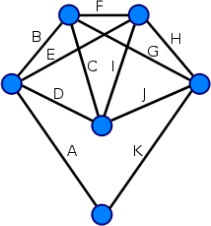
\includegraphics[width=0.3\columnwidth]{img/eulerian}
\end{center} 
We can transform the graph $H$ into a new graph $G$ (\textbf{De Bruijn graph}) in order to reduce the Hamiltonian path problem into the Eulerian path problem, which can be solved in \textbf{polynomial time}.

\paragraph*{De Bruijn graph G (dual of the graph of k-mers H).} A new graph $G$ is obtained from $H$ as follows:
\begin{itemize}
	\item $V_G$: set of all $(k-1)$-mers. Each k-mer of $H$ produces two $(k-1)$-mers in $G$, a prefix and a suffix.\\
	Example: $\verb|AAC|$ produces $\verb|AA|$ and $\verb|AC|$.
	\item $E_G$: an edge from node $u$ to node $v$ is in $G$ if and only if there exists a $k$-mer in $H$ containing $u$ as prefix and $v$ as suffix. Edges of $G$ represent $k$-mers, then an Eulerian path visiting each edge in $G$ exactly once gives a solution to the SBH problem.
\end{itemize}
Graph $G$ is called a \textbf{De Bruijn graph} (\textit{Euler graph}). Following our previous example:
\image{img/DeBruijn}{Example with Hamiltonian path and De Bruijn graph.}{0.8}
The unique Eulerian path of graph $G$ produces the sequence: $\verb|ATGTGCCGCA|$.\\
A possible problem that can be found is the fact that there can be more than one Eulerian path in the graph $G$. For example, considering the $3$-mers $\{\verb|ACT|, \verb|CTA|, \verb|TAC|\}$. We have two graphs:
\begin{center}
	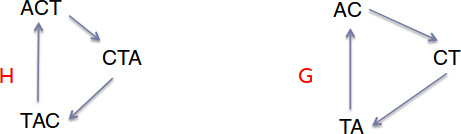
\includegraphics[width=0.7\columnwidth]{img/DeBruijn2}
\end{center} 
We can obtain three different sequences: $\verb|ACTAC|, \verb|TACTA| \text{ and } \verb|CTACT|$.\\
Each Eulerian path corresponds to a different DNA sequence, we can infer the sequence unambiguously if and only if the number of Eulerian paths in $G$ is exactly one.\\
Graph theory can supply:
\begin{itemize}
	\item Necessary and sufficient conditions for the existence of a Eulerian path in a graph.
	\item Necessary and sufficient conditions for the existence of a unique Eulerian path.
	\item Efficient algorithms for finding Eulerian paths in a graph.
\end{itemize}
SBH data contain errors caused by:
\begin{itemize}
	\item Hybridisation errors.
	\item Multiplicity errors.
\end{itemize}
Hybridisation errors give rise to:
\begin{itemize}
	\item \textbf{False negatives}: a k-mer appears in the sequence, but not in $H$.
	\item \textbf{False positives}: a k-mer does not appear in the sequence, but it is in $H$.
\end{itemize}

\section{De Bruijn graphs for assembly}
In 1995 it was proposed to use De Bruijn graphs for sequence assembly in the shotgun approach. The approach is usually called \textbf{De Bruijn approach}. The idea consists in decomposing each read of length $n$ into a set of $k$-mers: in a read of length $n$ there are $n-k+1$-mers.\\
Let $F=\{f_1, f_2, \dots, f_R\}$ be the set of reads. The \textbf{spectrum} is the set of all $k$-mers $w$ $(k=20,30)$:
$$\{(w,(i,i_{\alpha})) ~|~ w \in f_i, 1 \leq i \leq R\}$$
It means that $w$ occurs in read $f_i$ at position $i_{\alpha}$. The $k$-mer $w$ occurs $n(w)$ times in $F$ (\textit{coverage information}).
The De Bruijn approach follows these steps:
\begin{enumerate}
	\item Build the De Bruijn graph on the $k-1$-mers reporting on each edge the pair (read, position).
	\item Simplify the graph.
	\item Perform some variant of the Eulerian path to infer the sequences.
\end{enumerate}
It works well even in presence of errors. Reads with perfect overlaps induce a common path (a contig). Perfect overlaps are detected implicitly without any pairwise sequence alignment calculation.
\begin{center}
	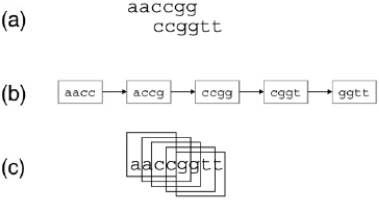
\includegraphics[width=0.7\columnwidth]{img/DeBruijn3}
\end{center} 
The pairwise alignment of the two reads in picture (\textit{a}) is a by-product of the graph construction (\textit{b}). The simple path through the graph implies a contig (\textit{c}).\\
Real sequencing data produce problems in overlap graphs and $k$-mer graphs:
\begin{itemize}
	\item \textbf{Spurs} are short, dead-end divergences from the main path. They are produced by sequencing error toward one end of a read. The error can be signalled by coverage dropping to zero.
	\begin{center}
		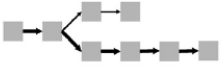
\includegraphics[width=0.4\columnwidth]{img/spurs}
	\end{center} 
	\item \textbf{Bubbles} are paths that diverge and then converge. They are produced by sequencing error toward the middle of a read, and by polymorphism in the target DNA. Efficient bubble detection is non-trivial.
	\begin{center}
		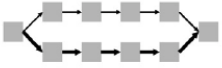
\includegraphics[width=0.4\columnwidth]{img/bubbles}
	\end{center} 
	\item Paths that converge and then diverge from the \textbf{frayed rope pattern}. They are produced by repeats in the target DNA.
	\begin{center}
		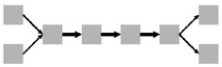
\includegraphics[width=0.4\columnwidth]{img/fragment}
	\end{center} 
	\item \textbf{Cycles} are paths that converge on themselves. They are produced by repeats in the target DNA. Through the associated info and number of occurrences of $k$-mers, it is possible to solve them.
\end{itemize}
All the described situations can occur together, creating a very complex graph structure.\\
Repetitions of a $k$-mer can occur:
\begin{itemize}
	\item \textbf{Within a single fragment in different locations (close):} when building the Eulerian path we make sure that edges corresponding to adjacent positions are visited successively. Moreover we can modify the Eulerian path construction by allowing multiple visits to the edges corresponding to repetitions.
	\item \textbf{As a repetitive regione in different fragmets (distant):} in this case the corresponding edge contains significantly more fragment positions than its non-repetitive neighbors.
\end{itemize} 
\paragraph*{De Bruijn approach: example.} Let's consider the sequence:
\begin{center}
	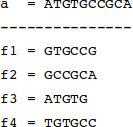
\includegraphics[width=0.2\columnwidth]{img/exampledeb}
\end{center} 
In this example we don't consider the complementary reads. For $K=3$ we have:
\begin{center}
	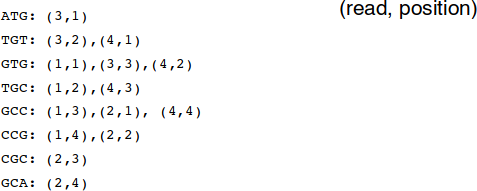
\includegraphics[width=0.8\columnwidth]{img/exampledeb2}
\end{center}
The corresponding Eulerian graph is:
\begin{center}
	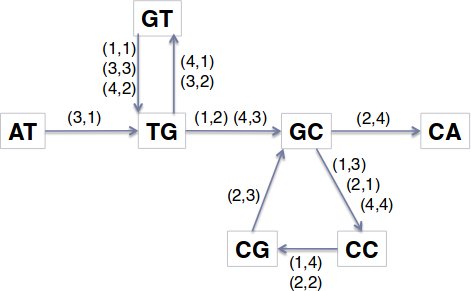
\includegraphics[width=0.7\columnwidth]{img/exampledeb3}
\end{center}

\section{Next Generation Sequencing}
New sequencing techniques have been developed, they allow for sequencing many DNA fragments in parallel, the new technologies are called \textbf{Next Generation Sequencing}. To sum up the improvement of this new technique we can see to these data:
\begin{itemize}
	\item \textbf{Sanger:} 1000bp, 100 reactions in parallel. Ten runs: 1 Mb.
	\item \textbf{NGS:} 50-500bp, millions of sequences in parallel. One run: 0,5-10 Gb.
\end{itemize}
NGS has an high throughput and a low cost, but on the other hand, it has less accuracy (less than 500 bp per read).\\
NGS has no need of cloning by means of virus or bacteria, no need of gel electrophoresis to discover the sequence of nucleotides. Sequencing is done step-by-step (pyrosequencing, sequencing by synthesis).

\paragraph*{Pyrosequencing.} Sequencing is performed by detecting each nucleotide incorporated by a DNA polymerase during DNA elongation. It relies on \textbf{light detection} each time a nucleotide is added.
\image{img/pyrosequencing}{Pyrosequencing approach.}{0.8}

\section{Sequencing Software}
Phred allows for assessing the quality of a DNA sequence on the basis of its electropherogram and by using statistical techniques. It compares the peaks and curves of sequenced fragments with the runs of well known sequences. It associate a quality value to each base.
\image{img/phread}{Phred execution.}{0.6}
Phred-score is the reliability value produced by Phred.

\section{Genome annotation}
With \textbf{genome annotation} we consider the fact of assigning identities and functions to sequences within the genome.\\
After sequencing there is the annotation phase, it requires many integrated tools for analysis and visualization of the sequenced genome. A main step is \textbf{gene inference}, it can happen through:
\begin{itemize}
	\item \textbf{Intrisic techniques:} protein-coding genes have recognizable features, there are several softwares to scan the genome and identify these features.
	\item \textbf{Estrinsic techniques:} comparison with known genomes and genes in other organisms.
	\item \textbf{Transcriptome analysis (RNA-seq):} an RNA sequence mirrors the sequence of the DNA from which it was transcribed. Consequently, by analyzing the entire collection of RNA sequences in a cell (\textit{transcriptome}), it is possible to determine when and where each gene is turned on or off in the cells and tissues of an organism. \textbf{RNA-seq} allows to quantify, discover and profile RNAs. 
\end{itemize}

\end{document}